%
% main.tex -- Paper zum Thema "Extreme Ereignisse"
%
% (c) 2018 Melina Staub, Hochschule Rapperswil
%
\chapter{Extreme Ereignisse\label{chapter:extrem}}
\lhead{Extreme Ereignisse}
\begin{refsection}
\chapterauthor{Melina Staub}
\definecolor{darkyellow}{rgb}{1,0.8,0}

\section{Einleitung}
\rhead{Einleitung}
Fast täglich erscheinen Schlagzeilen wie diese in der Zeitung:

\begin{itemize}
\item Wetter-Extreme häufen sich, auch in der Schweiz.
\item Seit Lothar wird es der vielleicht stärkste Sturm.
\index{Lothar}%
\item Die Schweiz reagiert empfindlich auf Wetteränderung.
\item Unwetter sorgten für eine chaotische Nacht.
\item Schweiz besonders stark vom Klimawandel betroffen.
\end{itemize}

Doch wieviel Wahrheit steckt in diesen Headlines? Sind sie nur Hirngespinste der Nachrichtenindustrie? Wollen uns die Medien täuschen oder geht da draussen wirklich etwas vor sich?

Dass die Natur im Wandel ist, steht ausser Frage. In der Geschichte der Erde waren extreme Ereignisse keine Seltenheit. Ob Eiszeiten, Trockenperioden oder lang anhaltender Regen, wohl jedes vorstellbare Ereignis ist vorgekommen. Vulkanausbrüche pumpten Kohlendioxid in die Atmosphäre und Meteoriteneinschläge lösten Tsunamis aus, die die Landflächen fluteten. Die Erde hat sich nach jedem Ereignis erholt und den neuen Umständen angepasst. Doch seit Mitte des 18. Jahrhunderts, im Zuge der Industrialisierung, hat sich viel verändert. Wald wurde verbrannt und in Ackerland umgewandelt, Dampfmaschinen erfunden und die Bevölkerungszahl explodierte. Waren es um 1750 noch knapp 1 Milliarde Menschen, betrug die Anzahl der Weltbevölkerung 200 Jahre später mehr als das Doppelte. Die Menschen begannen im grossen Stil CO$_2$ in die Atmosphäre auszustossen, was zum Treibhauseffekt führte. Dabei erwärmte sich die Globale Temperatur etwa 100 mal schneller, als sie das bei historischen natürlichen Klimaveränderungen getan hätte. Dies wurde bereits im Abschnitt \ref{skript:section:budyko} näher behandelt. 
\index{Eiszeit}%
\index{Meteoriteneinschlag}%
\index{Tsunami}%
\index{Industrialisierung}%
\index{Klimaveränderung}%

Die nachfolgenden Seiten wurden ohne Vorurteile oder frühzeitige Feststellungen rund um den Klimawandel erstellt. Am Ende soll die Wahrheit festgestellt werden.
Was bereits klar ist, die Erde wird den Klimawandel überstehen, wie sie auch schon extreme Trockenperioden oder Eiszeiten überstanden hat. Doch was wird aus uns, den Menschen?


\section{Was sind extreme Ereignisse?}
\rhead{Was sind extreme Ereignisse?}
Die Diskussionen um den Klimawandel erregt die Gemüter auf der ganzen Welt. Einige verleugnen ihn und andere verstehen ihn und tun alles um ihn zu stoppen. Besonders extreme Ereignisse, wie starke Regenfälle und die daraus resultierenden Überschwemmungen und Verwüstungen, Trockenperioden oder Wasserknappheit, bleiben in Erinnerung.
Eben diese Ereignisse weichen stark von den Durchschnittswerten ab und hinterlassen oft grosse Schäden und ebenso grosse Schadensummen.
Es stellt sich die Frage, ob diese extremen Ereignisse natürlichen Ursprungs sind, die Verteilung also durch den Zufall bestimmt wurde, ohne den Einfluss des Menschen oder ob diese auf den Klimawandel zurückzuführen sind und somit eine unnatürliche Häufung aufzeigen.


\subsection{Aufzeichnungen in der Schweiz}
In den {\em Schweizer Wetterjahresbüchern} und {\em Annalen der Schweizerischen Meteorologischen Zentralanstalt} lassen sich Wetter- und Klimadaten bis ins Jahr 1864 abrufen. Umfangreiche Tabellen und Berichte sind für Wetter- und Klimainteressierte ein historisch sehr bedeutender Datenschatz. 
Der Monatliche Wetterverlauf wurde ab dem Jahr 1911 geführt, extreme Wetterereignisse in Berichten beschrieben und aufgezeichnet (Abbildung \ref{Annalen}). Die Annalen wurden 2011 durch den Klimareport abgelöst, seit diesem Jahr sind der Klimabericht wie auch die Annalen für die Öffentlichkeit zugänglich und können Online eingesehen werden.
Mit diesen langen und genauen Klimadaten lässt sich tief in die Schweizer Klima-Vergangenheit blicken.

\begin{figure}
\centering
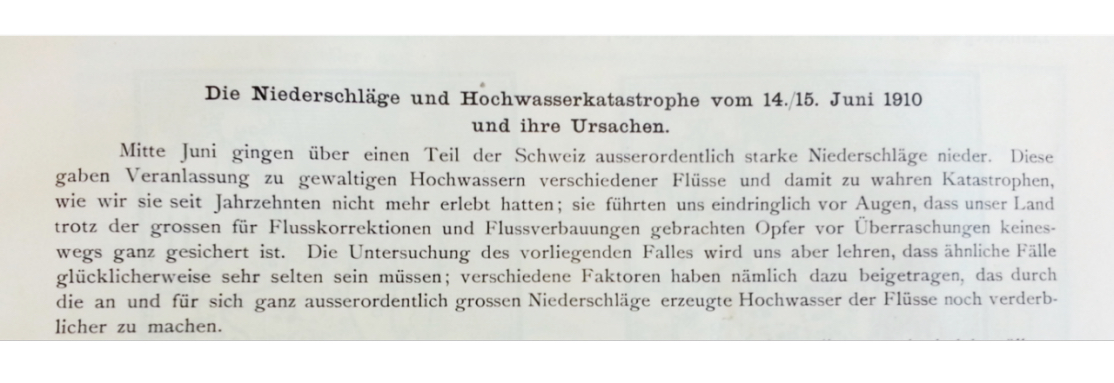
\includegraphics[width=\hsize]{extrem/Annalen.jpg}
\caption{Originaltext aus den Annalen 1910 zur Hochwasserkatastrophe vom Juni 1910. (Quelle: MeteoSchweiz)}
\label{Annalen}
\end{figure}


\subsection{Homogene Messreihen}
Die Modernisierung der Messgeräte, die Verschiebung der Messstandorte oder die Veränderung der Umgebung führen zu anderen Messwerten als beispielsweise diese des Vorgänger Messgeräts. Wenn man den Messstandort verlegt, verändert sich die Höhenlage. Dies wirkt sich auf die Temperaturmessung aus, da sich diese mit der Höhe im Mittel verschiebt. Temperaturverschiebungen zeichnen sich ab, die jedoch nichts mit dem Klima zu tun haben. Die Messergebnisse sind zwar genau, nicht aber miteinander vergleichbar, da die Höhenlage verändert wurde.
Dies bedeutet nicht, dass die alten Messgeräte ungenaue Messresultate lieferten, es bedeutet lediglich, dass die alten und neuen Messwerte nicht miteinander korrespondieren. 
Um die Klimadaten der letzten 150 Jahre miteinander vergleichen zu können, müssen die Messergebnisse vor dem Vergleich homogenisiert werden (Abbildung \ref{Homogen}), da die Daten ansonsten einen verfälschen Vergleich liefern.
Um diese Fehlinterpretationen zu vermeiden, sind in den {\em Schweizer Wetterjahresbüchern} und {\em Annalen der Schweizerischen Meteorologischen Zentralanstalt} sämtliche Messwerte homogenisiert worden. Ein direkter Vergleich ist nun möglich.

\begin{figure}
\centering
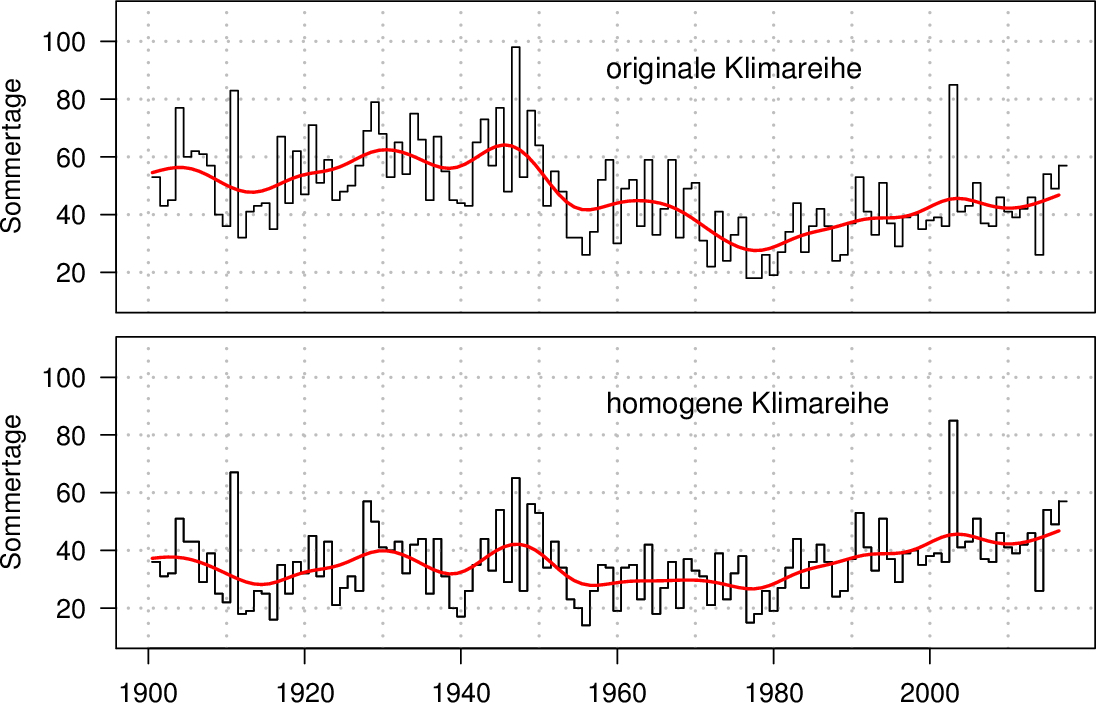
\includegraphics[width=0.6\textwidth]{extrem/Homogen.jpg}
\caption{Entwicklung der Anzahl Sommertage (Maximum--Temperatur $\ge 25^{\circ}$C ) pro Jahr an der Messstation Zürich/Fluntern seit 1901, gerechnet aus der originalen und homogenen Temperatur--Messreihe. Der geglättete Verlauf ist rot eingezeichnet. (Quelle: MeteoSchweiz)}
\label{Homogen}
\end{figure}

\begin{figure}
\centering
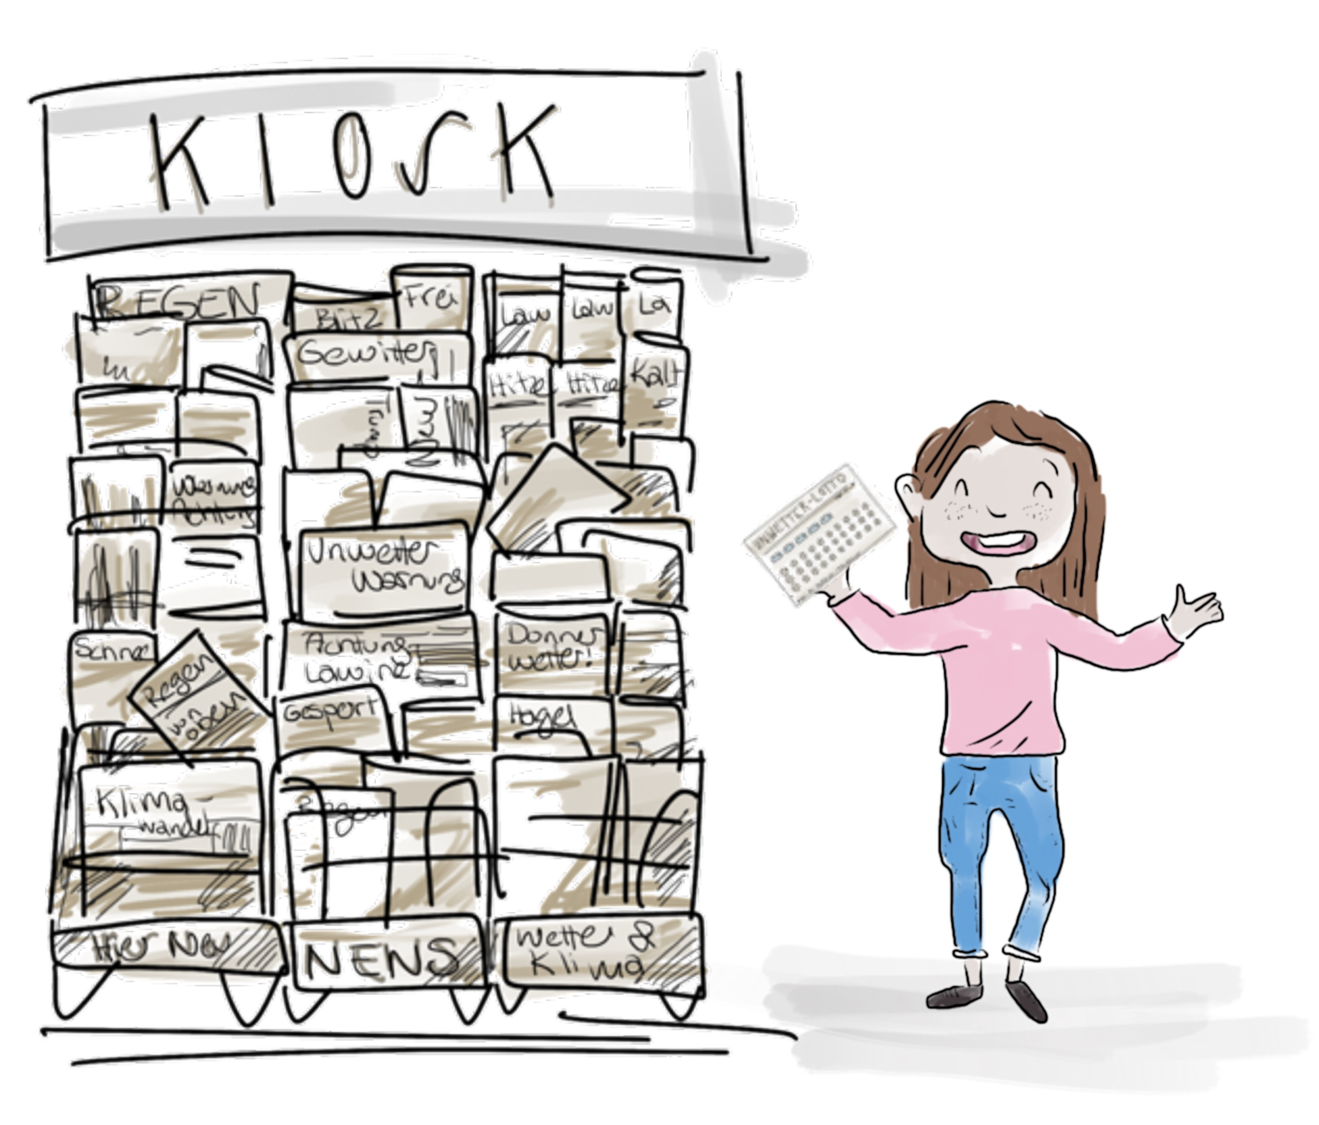
\includegraphics[width=0.4\textwidth]{extrem/Kiosk.pdf}
\caption{Unwetter-Lottoschein exklusiv erhältlich für MathSem Teilnehmer.}
\label{Kiosk}
\end{figure}


\section{Unwetter-Lotto}
\rhead{Unwetter-Lotto}
Um herauszufinden ob extreme Ereignisse nicht durch den Zufall bestimmt werden, benötigen wir vorerst ein Modell, um diese Berechnungen durchführen zu können.
Hierbei bedienen wir uns eines Glücksspiels, genauer gesagt des Lottos.

Exklusiv für die Leserinnen und Leser dieses Seminarbuches steht der Unwetter-Lottoschein zur Verfügung, welchen man am Zeitungskiosk (Abbildung \ref{Kiosk}) erwerben und statt auf Zahlen, auf Unwetterereignisse tippen kann. Auf dem Unwetter-Lotto-Schein (Abbildung \ref{Lottoschein}) können wie beim normalen Zahlenlotto verschiedene Zahlen ausgewählt und seine Tipp abgeben werden. Danach gibt es eine Unwetterziehung und man kann seine abgegebenen Tipps mit der Ziehung vergleichen.

\begin{figure}
\centering
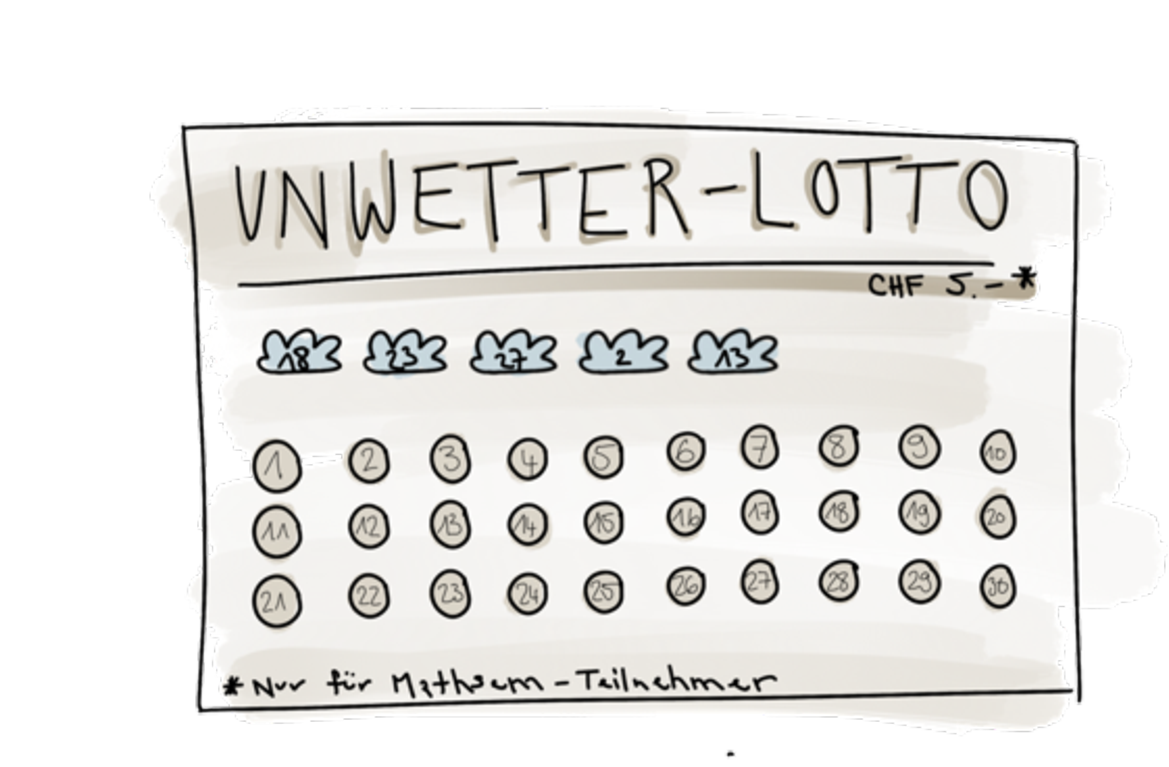
\includegraphics[width=0.7\textwidth]{extrem/Lottoschein.pdf}
\caption{Unwetter-Lottoschein.}
\label{Lottoschein}
\end{figure}

Die Anzahl Kugeln 1--30 beschreiben alle vorhandenen Ereignisse,
welche wir \textcolor{red}{\textbf{N}} nennen. Die fünf Wolken
stehen für die Anzahl Tipps (Kreuze), welche wir abgeben dürfen.
Das heisst, welche Unwetter \textcolor{blue}{\textbf{n}} wir aus
den totalen Ereignissen 1--30 ($\textcolor{red}{\textbf{N}}=30$)
auswählen können. Die bei der Unwetterziehung gezogene Anzahl Ereignisse
\textcolor{green}{\textbf{M}} sind unsere Stichprobe aus allen
Ereignissen (Abbildung \ref{ErklaerungLotto}). Wie die Unwetterziehung
funktioniert und wie sie mit dem Klimawandel in Verbindung gebracht
wird, ist später im Abschnitt~\ref{UnwetterVert} näher erklärt.

Jetzt stellen wir uns die entscheidende
\newtheorem{frage}[satz]{Frage}
\begin{frage}
Wie wahrscheinlich ist es, \textcolor{darkyellow}{\textbf{k}} richtige
im Unwetter-Lotto (Abbildung \ref{WahrscheinlichkeitUnwetter-Lotto})zu
erhalten?
\end{frage}
Wir bezeichnen mit $X$ die Anzahl der erzielten Richtigen,
die gesuchte Wahrscheinlichkeit ist dann $P(X=k)$.

\begin{figure}
\centering
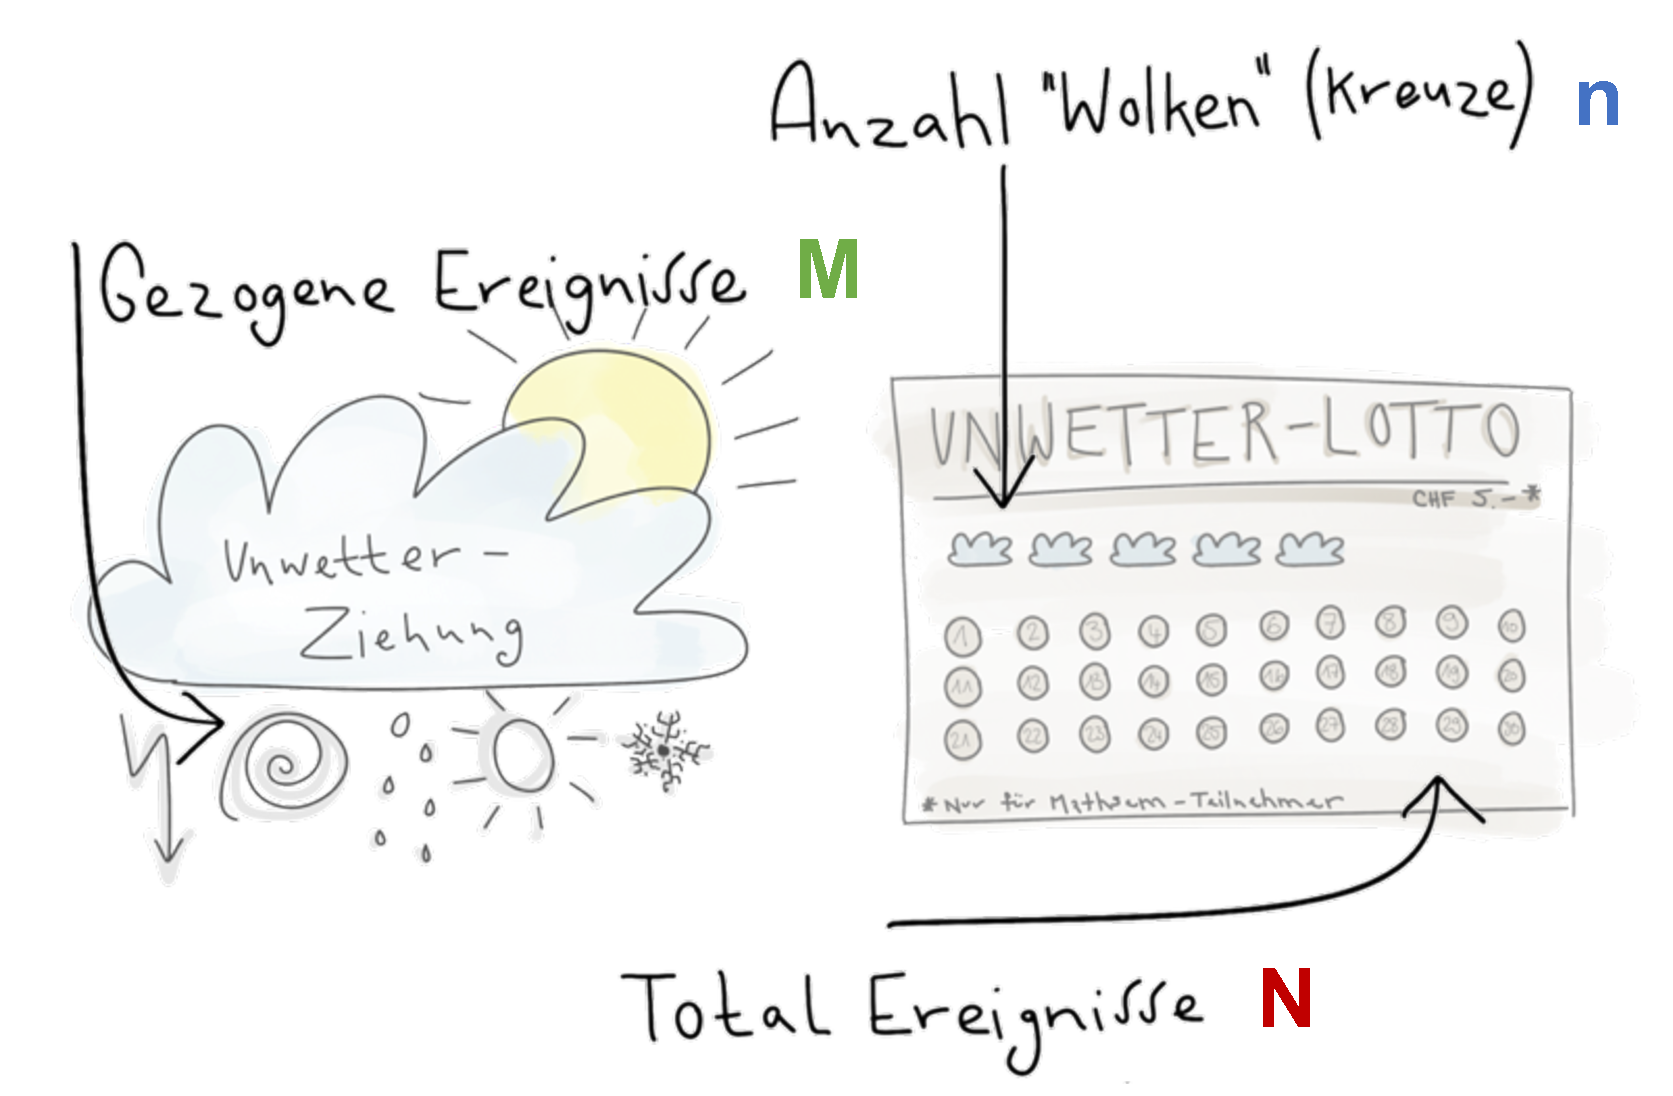
\includegraphics[width=0.6\textwidth]{extrem/Lottoscheinausgefuellt.pdf}
\caption{Unwetter-Lottoschein mit den Variabeln und der Unwetterziehung.}
\label{ErklaerungLotto}
\end{figure}

\begin{figure}
\centering
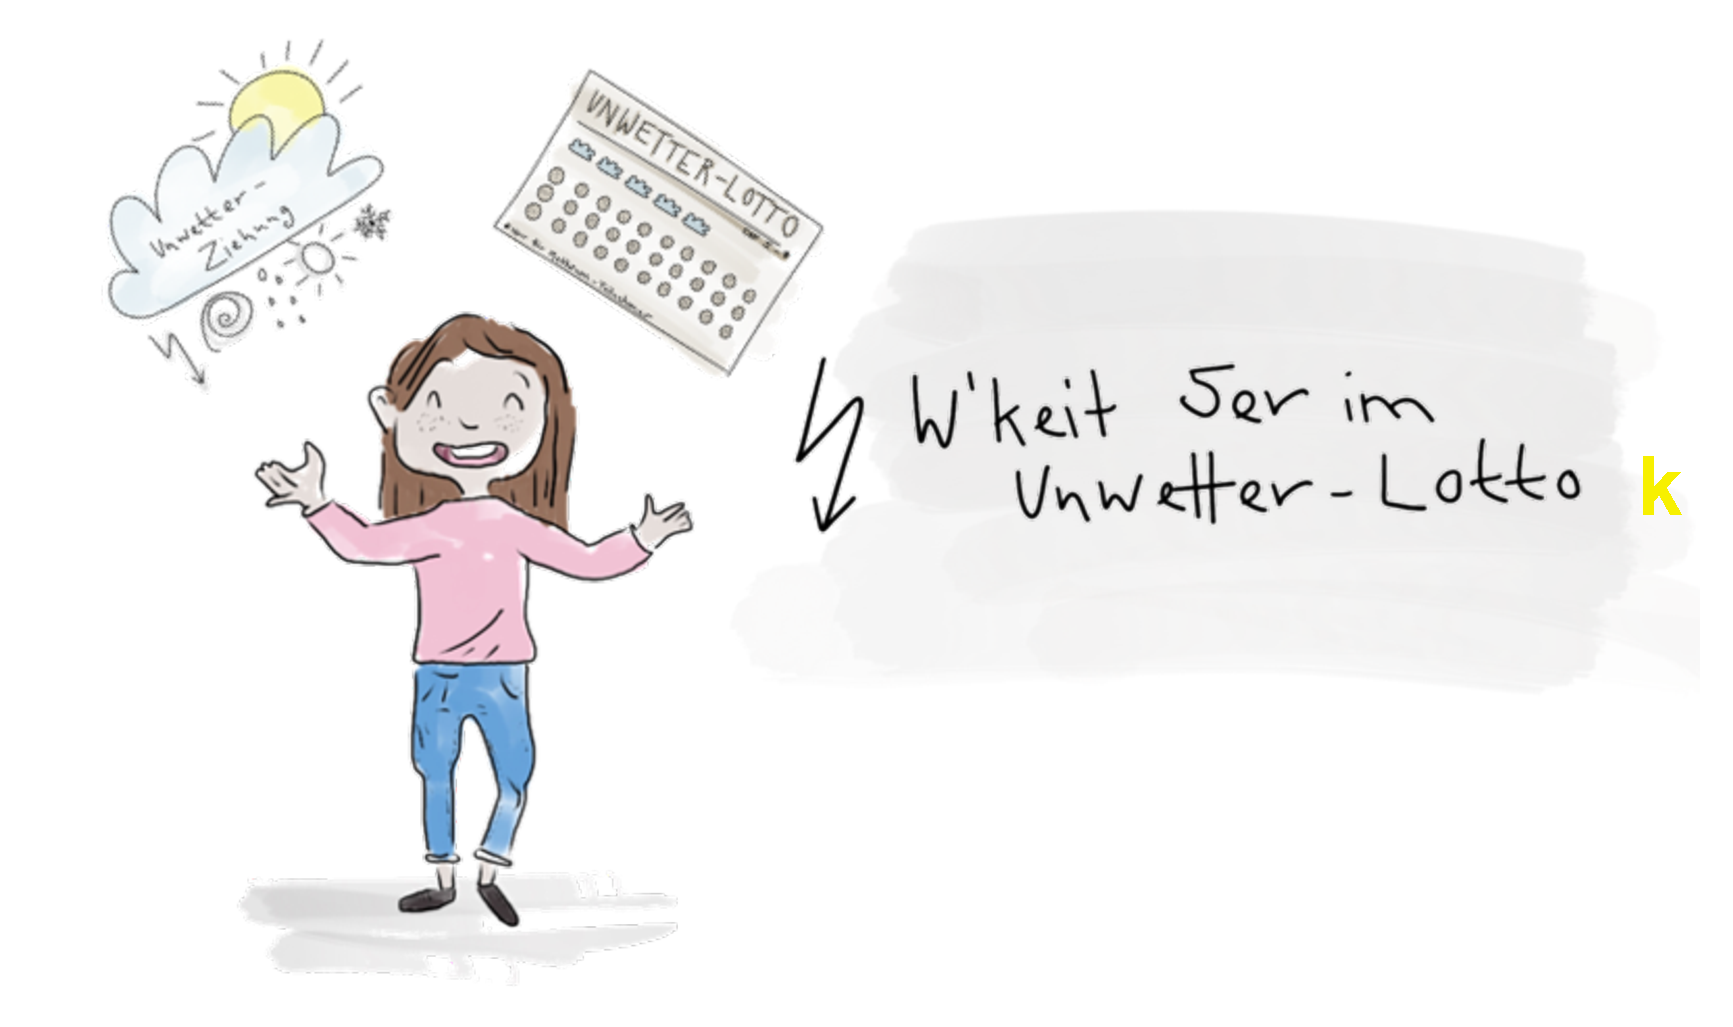
\includegraphics[width=0.6\textwidth]{extrem/wkeitlotto.pdf}
\caption{Wahrscheinlichkeit, einen 5er im Unwetter-Lotto zu erhalten.}
\label{WahrscheinlichkeitUnwetter-Lotto}
\end{figure}


\subsection{Lottoproblem} \label{Lottoproblem}
\index{Lottoproblem}
Mit dem Unwetter-Lotto wurde das bekannte Lottoproblem beschrieben
--- ein Experiment ohne zurücklegen. Mit jeder Ziehung ändert sich
im Laufe des Experiments die Grundgesamtheit und somit auch die
Wahrscheinlichkeit, ein bestimmtes Ereignis zu ziehen. Der Ziehmodus
ist vorgegeben und somit ist auch der Gewinn bekannt. Das Lottoproblem
ist somit nichts anderes als die hypergeometrische Verteilung
\begin{equation}
P(X = k) = 
\frac{\displaystyle \binom{M}{k} \binom{N-M}{n-k}}{\displaystyle \binom{N}{n} }. 
\label {V1}
\end{equation}

Die hypergeometrische Verteilung \eqref{V1} beschreibt die Wahrscheinlichkeit aus $N$ gegebenen Elementen, mit $n$ Elementen einer speziellen Eigenschaft, und einer Stichprobe aus $M$ Elementen genau $k$ Treffer zu erzielen. 
Anders als die Binomialverteilung ist die hypergeometrische Verteilung ein Experiment ohne Zurücklegen. Die Wahrscheinlichkeit ändert sich mit jeder Ziehung. 
%
Das oben beschriebene Lottoproblem beziehungsweise die hypergeometrische
Verteilung liefert uns folgende Fragestellung:
\index{hypergeometrische Verteilung}%

Wie wahrscheinlich ist es...

\begin{itemize}
\item \dots auf einem Lottozettel mit \textcolor{red}{\textbf{N}} Feldern \dots
\item \dots auf welchem man \textcolor{blue}{\textbf{n}} Unwetter ankreuzen kann \dots
\item \dots und bei der Ziehung \textcolor{green}{\textbf{M}} Unwetter gezogen werden \dots
\item \dots genau \textcolor{darkyellow}{\textbf{k}} Richtige zu haben?
\end{itemize}

Je tiefer die Wahrscheinlichkeit ausfällt, desto unwahrscheinlicher
ist es, dass Unwetter \textcolor{green}{\textbf{M}} bei der
Unwetterziehung gezogen werden. Dies ist dann der Fall, wenn die
Wahrscheinlichkeit mehrerer Unwetter gefragt ist. Die Frage wie
wahrscheinlich (\textcolor{darkyellow}{\textbf{k}}) es ist, dass aus
\textcolor{red}{\textbf{N}} Feldern auf dem Lottozettel, genau
\textcolor{blue}{\textbf{n}} Unwetter welche man ankreuzen darf,
\textcolor{green}{\textbf{M}} gezogen werden, kann nun beantwortet
werden.


\section{Die Unwetter-Verteilung} \label{UnwetterVert}
\rhead{Die Unwetter-Verteilung}
Um die Frage zu beantworten, ob sich das Klima verändert und ob immer häufiger extreme Ereignisse auftreten, bedienen wir uns dem Werkzeugkasten der Statistik. Mit dem im Abschnitt genannten \ref{Lottoproblem} lässt sich die Unwetter-Verteilung aufstellen. Die Fragestellung muss dabei ein wenig auf unser Problem angepasst werden.

Dabei beziehen sich die \textcolor{red}{\textbf{N}} Felder auf dem Lottozettel auf die Anzahl Jahre mit zugehörigen Messwerten. Die Anzahl Unwetter \textcolor{blue}{\textbf{n}} welche man ankreuzen kann, sind die extremen Ereignisse, also Unwetter oder Messungen welche besonders extrem ausgefallen sind. Die Ziehung der \textcolor{green}{\textbf{M}} Unwetter ist unser Beobachtungszeitraum. Im nachfolgenden Beispiel wird ein Beobachtungszeitraum von 10 Jahren angenommen. Je tiefer die Wahrscheinlichkeit ausfällt, desto unwahrscheinlicher ist es, dass viele extreme Ereignisse in den letzten 10 Jahren \textcolor{green}{\textbf{M}} vorgekommen sind. Die Frage die nun beantwortet werden muss lautet:

\begin{frage}
Wie wahrscheinlich
ist es, dass von \textcolor{blue}{\textbf{n}} extremen Ereignissen
aus einer Messreihe von \textcolor{red}{\textbf{N}} Jahren,
\textcolor{darkyellow}{\textbf{k}}
in den
letzten 10 Jahren (\textcolor{green}{\textbf{M}}) vorkommen?
\end{frage}

\begin{figure}
\centering
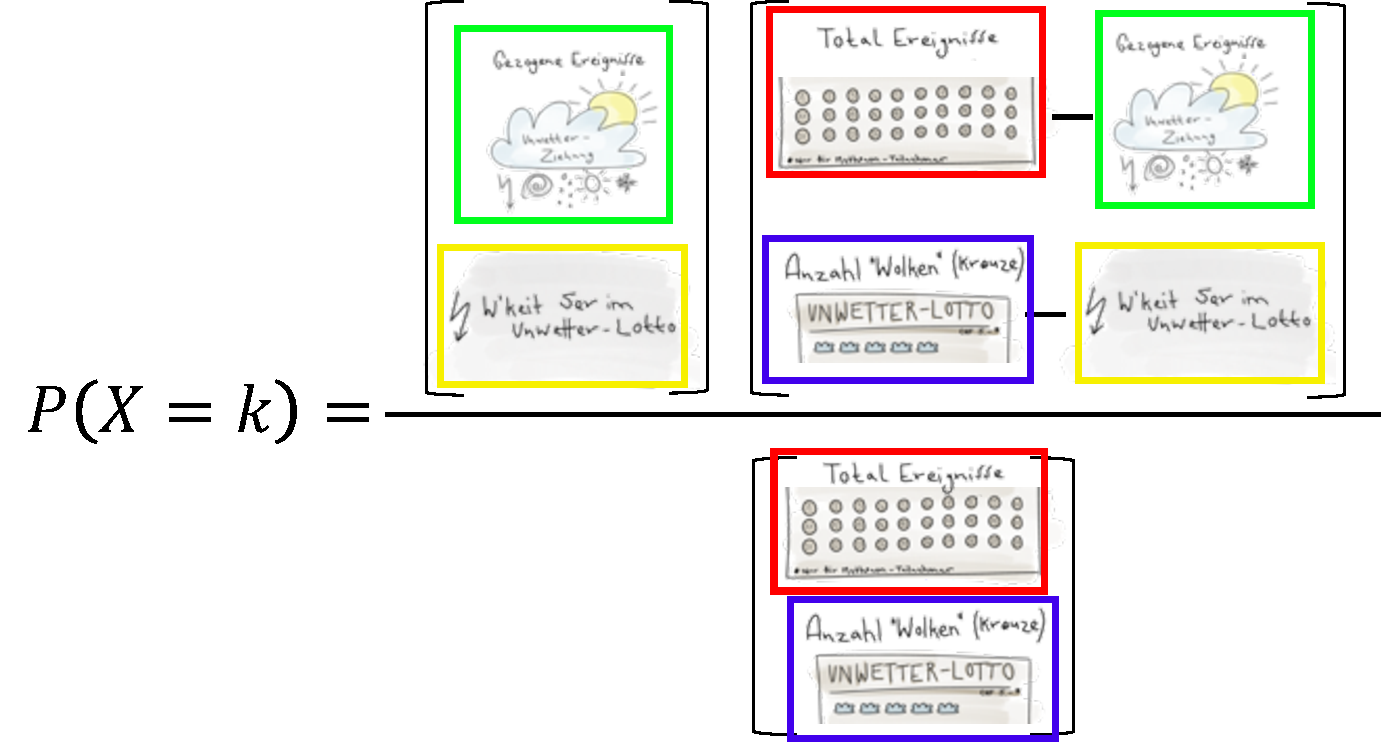
\includegraphics[width=0.6\textwidth]{extrem/Unwettervert.pdf}
\caption{Die Unwetter-Verteilung. Die Wahrscheinlichkeit sagt aus, wie wahrscheinlich es ist n extreme Ereignisse aus einer Messreihe von N Jahren in den letzten 10 Jahren (M) vorzufinden.}
\label{UnwetterVerteilung}
\end{figure}


\subsection{Beispiel} \label{Beispiel}
Die hypergeometrische Verteilung setzt sich aus verschiedenen Binomialkoeffizienten

\begin{align*}
\binom{n}{k} = \frac {n!}{k! \cdot (n-k)!} 
\end{align*}
zusammen.

Um im Abschnitt~\ref{MesspunkteSchweiz} die Klimadaten auszuwerten, werden im nachfolgenden Beispiel der hypergeometrischen Verteilung die folgenden Werte für die entsprechenden Variabeln verwendet:
\begin{align*}
N&=75&&\text{Anzahl Jahre der Messreihe}\\
M&=10&&\text{letzte 10 Jahre der Messreihe}\\
n&=7&&\text{7 ausgewählte Ereignisse (extreme Ereignisse)}\\
k&=3&&\text{3 extreme Ereignisse (welche eintreffen)}
\end{align*}

Die Wahrscheinlichkeit $P(X=3)$ ergibt sich aus:
Anzahl der Möglichkeiten, genau 3 extreme Ereignisse (und damit genau 4 normale Ereignisse) auszuwählen, dividiert durch die Anzahl Möglichkeiten 7 Ereignisse aus allen Ereignissen auszuwählen. Dabei gibt es
\begin{align*}
\binom{M}{k} = \binom{10}{3} = 120
\end{align*}
%
Möglichkeiten, genau 3 extreme Ereignisse auszuwählen.
Zudem gibt es 
\begin{align*}
\binom{N-M}{n-k} = \binom{75-10}{7-3} = \binom{65}{4} = 677040
\end{align*}
%
Möglichkeiten, genau 4 normale Ereignisse auszuwählen.
Da jede Möglichkeit 3 extreme Ereignisse mit jeder Möglichkeit 4 normale Ereignisse auszuwählen kombiniert werden kann, ergeben sich
\begin{align*}
\binom{M}{k} \cdot \binom{N-M}{n-k} = \binom{10}{3} \cdot \binom{75-10}{7-3} = 120 
\cdot 677040 = 81244800
\end{align*}
%
Möglichkeiten für genau 3 extreme und 4 normale Ereignisse auszuwählen.
Zusätzlich gibt es insgesamt
\begin{align*}
\binom{N}{n} = \binom{75}{7} = 1984829850
\end{align*}
%
Möglichkeiten, 7 Ereignisse aus allen Ereignissen zu ziehen.
Für k=3 erhalten wir somit die Wahrscheinlichkeit
\begin{equation}
P(X = 3) = \frac{\displaystyle \binom{M}{k} \binom{N-M}{n-k}}{\displaystyle \binom{N}{n} }  \\
= \frac{\displaystyle \binom{10}{3} \binom{75-10}{7-3}}{\displaystyle \binom{75}{7} } \\
= \frac{ 120 \cdot 677040}{ 1984829850 } = 0.0409329.
\label {V2}
\end{equation}
%
In 4.09 \% aller Fälle werden genau 3 extreme und 4 normale Ereignisse vorkommen. Diese Berechnung lässt sich mit allen $X=k$ durchführen, dies wird im Abschnitt~\ref{Dichtehyper} gemacht.


\subsection{Die hypergeometrische Verteilung} \label{Dichtehyper}
Im vorangehenden Beispiel \eqref{V2} wurde die Wahrscheinlichkeit der hypergeometrischen Verteilung berechnet für $P(k = 3)$. 

\begin{definition}
Die hypergeometrische Verteilung, sind die Wahrscheinlichkeitswerte für alle P(X=k).
\end{definition}

\begin{table}
\centering
\begin{tabular}{>{$}c<{$}|>{$}l<{$}}
k&P(X=k)\\
\hline
0&0.3507558\\
1&0.4161509\\
2&0.1872679\\
3&0.0409329\\
4&0.0046214\\
5&0.0002640\\
6&6.87\cdot 10^{-6}\\
7&6.04\cdot 10^{-8}
\end{tabular}
%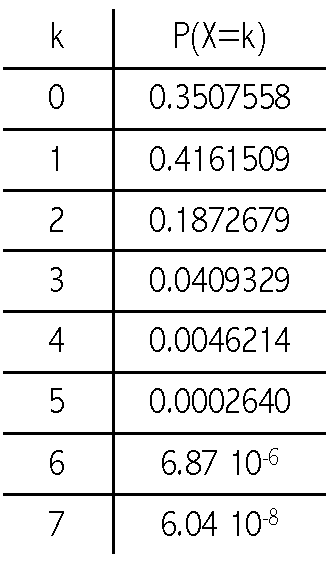
\includegraphics[width=0.2\textwidth]{extrem/TabHyperV.pdf}
\caption{Wahrscheinlichkeiten $P(X=k)$ der verschiedenen Ereignisse, beschreiben unsere hypergeometrische Verteilung.}
\label{TabHyperV}
\end{table}

Für alle $P (X=k)$ ergeben sich folgende Wahrscheinlichkeiten (Abbildung \ref{TabHyperV}). Die Wahrscheinlichkeit beschreibt dabei, wie wahrscheinlich es ist, genau k extreme Ereignisse in den letzten 10 Jahren vorzufinden.
Beachten Sie, dass die Werte N, M und n das Experiment beschreiben und nicht mehr verändert werden. Die Variable k hingegen kann alle möglichen Ausgänge des Experiments annehmen, in unserem Beispiel also von 0 bis 7.

\begin{figure}
\centering
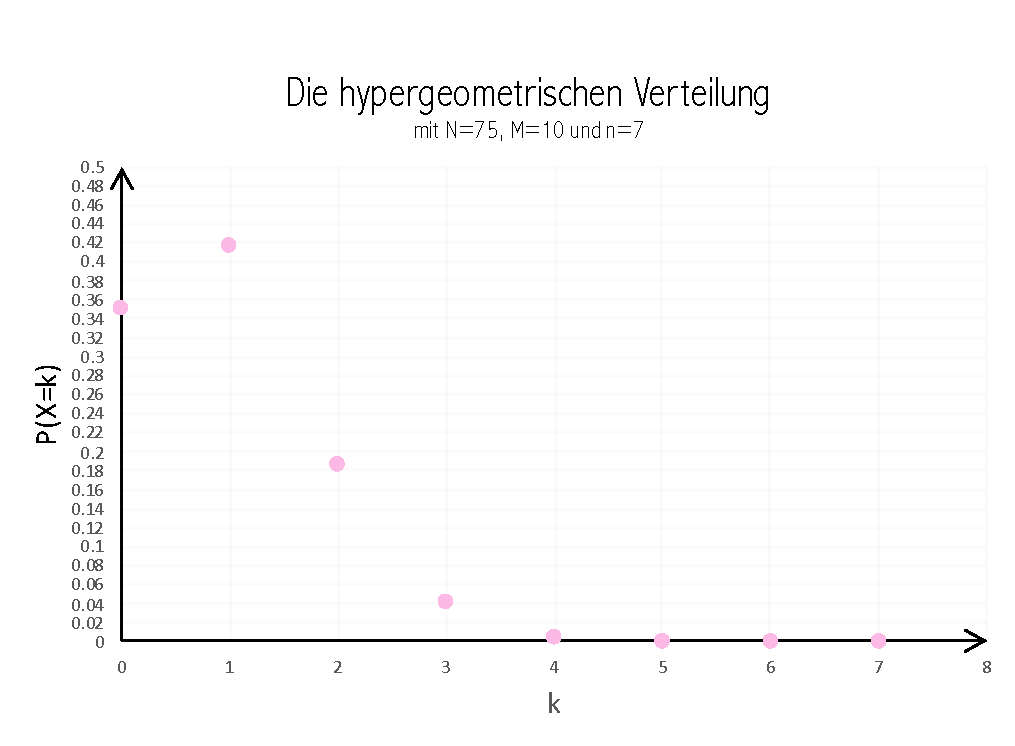
\includegraphics[width=0.8\textwidth]{extrem/HyperV.pdf}
\caption{Die hypergeometrische Verteilung unseres Beispiels. Sie
zeigt auf, wie wahrscheinlich es ist, genau k extreme Ereignisse
in den letzten 10 Jahren vorzufinden.}
\label{HyperV}
\end{figure}

In Abbildung \ref{HyperV} ist sehr gut ersichtlich, dass die Wahrscheinlichkeit bei genau einem extremen Ereignis in den letzten 10 Jahren am höchsten ist. Wohingegen genau 3 Ereignisse nur noch eine Wahrscheinlichkeit von 4.09\% aufweisen, was bereits sehr unwahrscheinlich ist. Häufungen von Ereignissen, welche die Anzahl 3 überschreiten, sind so unwahrscheinlich, dass sie kaum natürlichen Ursprungs sein können.

\subsection{Sind viele extreme Ereignisse wahrscheinlich?}
Stellt man sich nun die Frage, ob viele extreme Ereignisse wahrscheinlich sind, muss berechnet werden wie wahrscheinlich es ist $k$ oder mehr Ereignisse in den letzten 10 Jahren ($M$) zu erhalten. 
Die Verteilungsfunktion der hypergeometrischen Verteilung ist nichts anderes als die aufsummierte Wahrscheinlichkeit aller möglichen Ausgänge. Weil für unser Beispiel aber wichtig ist, wie wahrscheinlich es ist, drei oder mehr extreme Ereignisse in den letzten 10 Jahren vorzufinden, muss die komplementäre Verteilungsfunktion der hypergeometrischen Verteilung
\begin{align*}
F(x) = P(X \ge I ) = \sum \limits_{k=I}^n P(X = k)
\end{align*}
%
angewendet werden (Abbildung \ref{HyperExt}). 
Möchten wir die Wahrscheinlichkeit wissen, drei oder mehr extreme Ereignisse in den letzten 10 Jahren vorzufinden, müssen die einzelnen Wahrscheinlichkeiten aufsummiert \eqref{V3} und werden
%
\begin{equation}
\begin{aligned}
\bar{F}(3) &=  P(X \ge 3) \\
&= P(X = 3) + P(X = 4) + P(X = 5) + P(X = 6) + P(X = 7) \\
&= 0.0409329 + 0.0046214 + 0.00026340 + 6.87 10^{ -6 } + 6.04 10^{ -8 } \\
&= 0.045833 = 4.58\%.
\label{V3}
\end{aligned}
\end{equation}
%
Drei oder mehr extreme Ereignisse in den letzten 10 Jahren sind mit einer Wahrscheinlichkeit von 4.58\% möglich. 
Die Wahrscheinlichkeit ein oder zwei extreme Ereignisse in den letzten 10 Jahren zu haben ist mit 64.49\% und 23.30\% relativ hoch. Ab drei oder mehr Ereignissen nimmt die Wahrscheinlichkeit rasant ab und wird ohne äussere Einflüsse und Einwirkungen sehr unwahrscheinlich und ab 5 oder mehr Ereignissen nahezu unmöglich.
%
\begin{table}
\centering
\begin{tikzpicture}[>=latex,thick]
\fill[color=red!20]
	(-1.64,-1.92)--
	(0.3,-1.92)--
	(0.3,-0.18)--
	(2.2,-0.18)--
	(2.2,0.25)--
	(-1.64,0.25)--cycle;
\node at (0,0) {\begin{tabular}{ >{$}l<{$}| >{$}l<{$}| >{$}l<{$}}
k&P(X=k)&P(X\ge k)\\
\hline
0& 0.3507558        & 1.000000         \\
1& 0.4161509        & 0.649244         \\
2& 0.1872679        & 0.233093         \\
3& 0.0409329        & 0.045833         \\
4& 0.0046214        & 0.004892         \\
5& 0.0002640        & 0.000271         \\
6& 6.87\cdot 10^{-6}& 6.93\cdot 10^{-6}\\
7& 6.04\cdot 10^{-8}& 6.04\cdot 10^{-8}\\
\end{tabular}
};
\end{tikzpicture}
%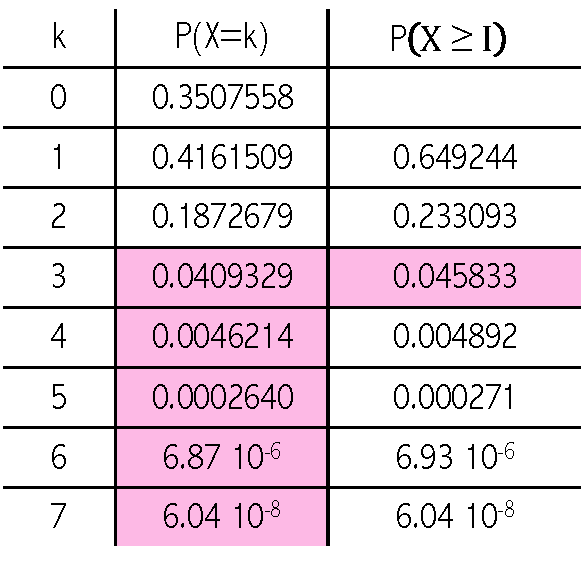
\includegraphics[width=0.3\textwidth]{extrem/TabExt.pdf}
\caption{Wahrscheinlichkeit $P(X = k)$ aller Ereignisse unseres
Beispiels und die Wahrscheinlichkeiten $P(X \ge k)$ der komplementären
Verteilfunktion. Die Rosa markierten Felder sind die Werte, die zur
Berechnung in \ref{Beispiel}) gebraucht wurden. }
\label{TabExt}
\end{table}

\begin{figure}
\centering
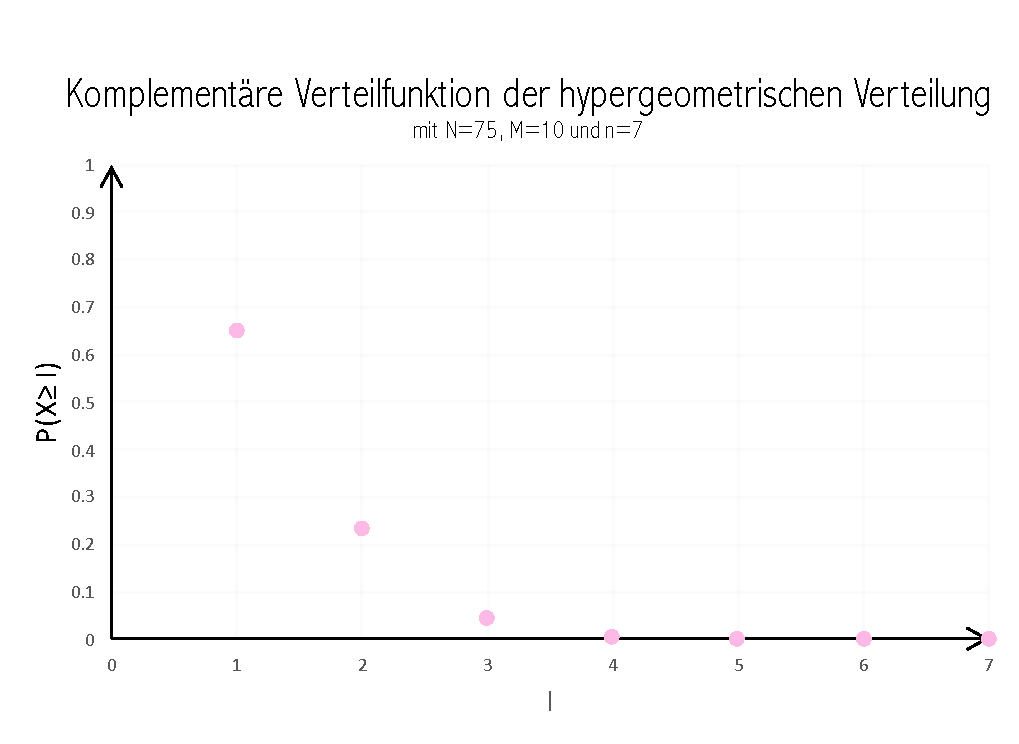
\includegraphics[width=0.8\textwidth]{extrem/HyperExt.pdf}
\caption{Die komplementäre Verteilfunktion $\bar{F}(x)$ der hypergeometrischen Verteilung zeigt auf, wie wahrscheinlich es ist mehr als k Ereignisse in den letzten 10 Jahren vorzufinden.}
\label{HyperExt}
\end{figure}

\section{Hypothesentest}
\index{Hypothesentest}
\rhead{Hypothesentest}
Hypothesentests werden immer dann durchgeführt, wenn aus erhobenen Daten etwas nachgewiesen werden muss, zum Beispiel, dass sich extreme Ereignisse in den letzten Jahren häuften. Der Grundsatz bei allen statistischen Tests ist, dass das Gegenteil widerlegen werden muss - wir müssen also widerlegen, dass extreme Ereignisse in den letzten Jahren zufällig verteilt sind. Die Nullhypothese wäre also: Die Häufung von extremen Ereignissen entscheidet der Zufall und werden nicht beeinflusst. Kurz: Es findet kein Klimawandel statt.
Zu vergleichen ist ein Hypothesentest mit einer Gerichtsverhandlung, die Nullhypothese wäre in diesem Fall: Der Angeklagte ist {\em nicht schuldig}. Es wird also vorerst das Gegenteil von dem behauptet, was man widerlegen möchte. Daher muss davon ausgegangen werden, dass die Nullhypothese stimmt, bis das Gegenteil bewiesen wurde. Hierfür benötigt es genügend Beweise, welche die {\em nicht Schuld} oder hier die Nullhypothese widerlegen können.
Falls ungenügend viele Beweise vorliegen, muss davon ausgegangen werden, dass die Hypothese stimmt oder eben der Angeklagte {\em nicht schuldig} ist. Dies bedeutet aber keinesfalls, dass der Angeklagte auch kein Verbrechen begangen hat. Wenn zu wenige Beweise vorliegen, heisst das nur, dass man die Schuld des Angeklagten nicht beweisen kann. Erst wenn die Nullhypothese widerlegt werden kann, und somit die Schuld bewiesen wird, ist der Angeklagte schuldig.


\subsection{Nullhypothese}
Unsere Nullhypothese, die geprüft werden soll:

\begin{quote}
In den letzten Jahren gab es keinen Wandel oder eine Häufung von extremen Ereignissen.
\end{quote}
oder:
\begin{itemize}
\item Das Klima verändert sich nicht
\item Alles bleibt beim Alten
\item Der Zufall bestimmt die Anordnung der (extremen) Ereignisse
\end{itemize}
%
Diese Nullhypothese gilt es nun zu widerlegen, um den Klimawandel zu beweisen.


\subsection{Signifikanzniveau}
\index{Signifikanz}
Die Grenze für die Widerlegung der Nullhypothese beschreibt die statistische Signifikanz $\alpha$. Über diesen Wert wird eine bestimmte Irrtumswahrscheinlichkeit festgelegt.
Bei der Festlegung dieser Schwelle wird bedacht, was für Konsequenzen es hätte, dass ein beobachteter Unterschied nur zufällig erfolgt. Sind die Folgen gravierend, wählt man eher ein tiefes Niveau (1 \% statt 5\%).

Bei einem Medikament wird daher eher ein tiefes Signifikanzniveau gewählt. Als Vergleich, beim Nachweis der Existenz des Higgs-Bosons\footnote{%
Das Higgs-Boson ist Elementarteilchen (Benannt nach dem britischen Physiker Peter Higgs), deren Existenz wurde im Juli 2012 durch das CERN (mit dem Larce Hadron Collider LHC) bestätigt.} wurde ein noch viel strengeres Kriterium gewählt, es entspricht einem Wert von 1 in 3.5 Millionen. 

Da extreme Ereignisse nicht direkt lebensbedrohlich sind, wird im Folgenden $\alpha$ = 5\% gewählt.
Falls die Nullhypothese richtig ist, darf die Wahrscheinlichkeit dafür, dass sie fälschlicherweise abgelehnt wird, nicht unter 5\% fallen (Abbildung \ref{SigniAlpha}).


Eine Häufung von 3 oder mehr extremen Ereignissen wären nicht mehr durch den Zufall bestimmt. Das bedeutet, wenn von den 7 extremsten Ereignissen der letzten 75 Jahre 3 oder mehr in den letzten 10 Jahren waren, müssen wir auf den Klimawandel schliessen. Die Nullhypothese wäre ohne Zweifel widerlegt.

\begin{figure}
\centering
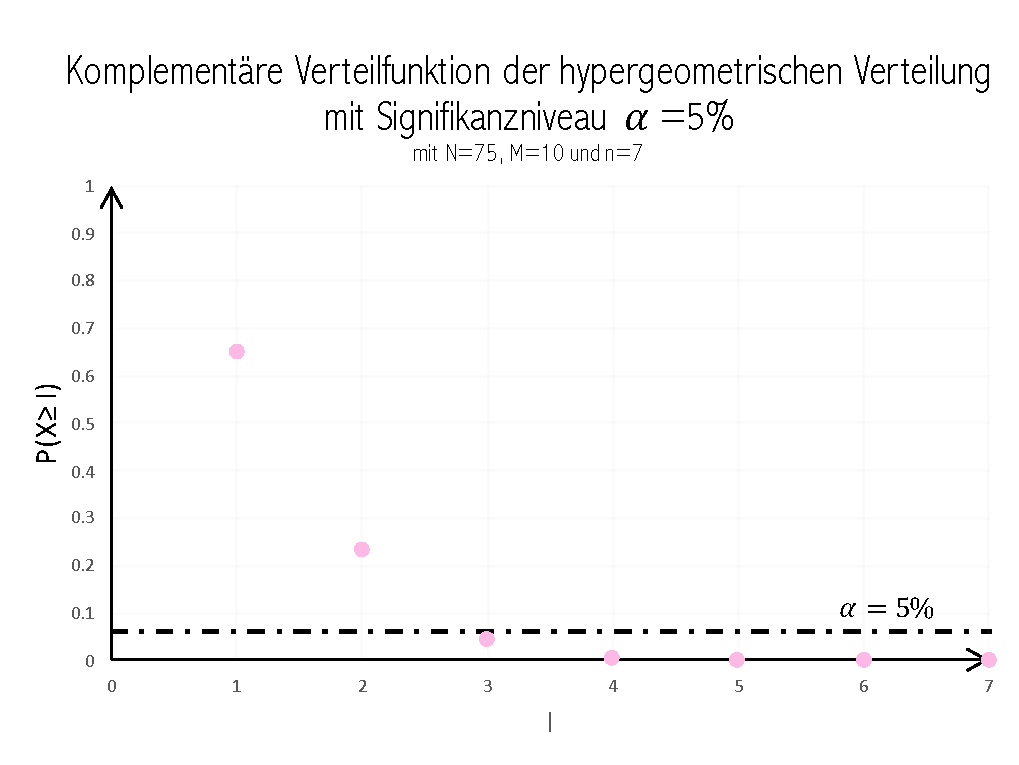
\includegraphics[width=0.8\textwidth]{extrem/SigniAlpha.pdf}
\caption{Die komplementäre Verteilfunktion der hypergeometrischen Verteilung mit dem eingezeichneten Signifikanzniveau von 5\%.}
\label{SigniAlpha}
\end{figure}


\section{Messpunkte Schweiz} \label{MesspunkteSchweiz}
\rhead{Messpunkte Schweiz}
Um eine möglichst grosse Vielfalt von Messreihen zu bekommen, werden verschiedene Messpunkte in der Schweiz (Abbildung~\ref{MesspunkteCH}) angeschaut. 

\begin{figure}
\centering
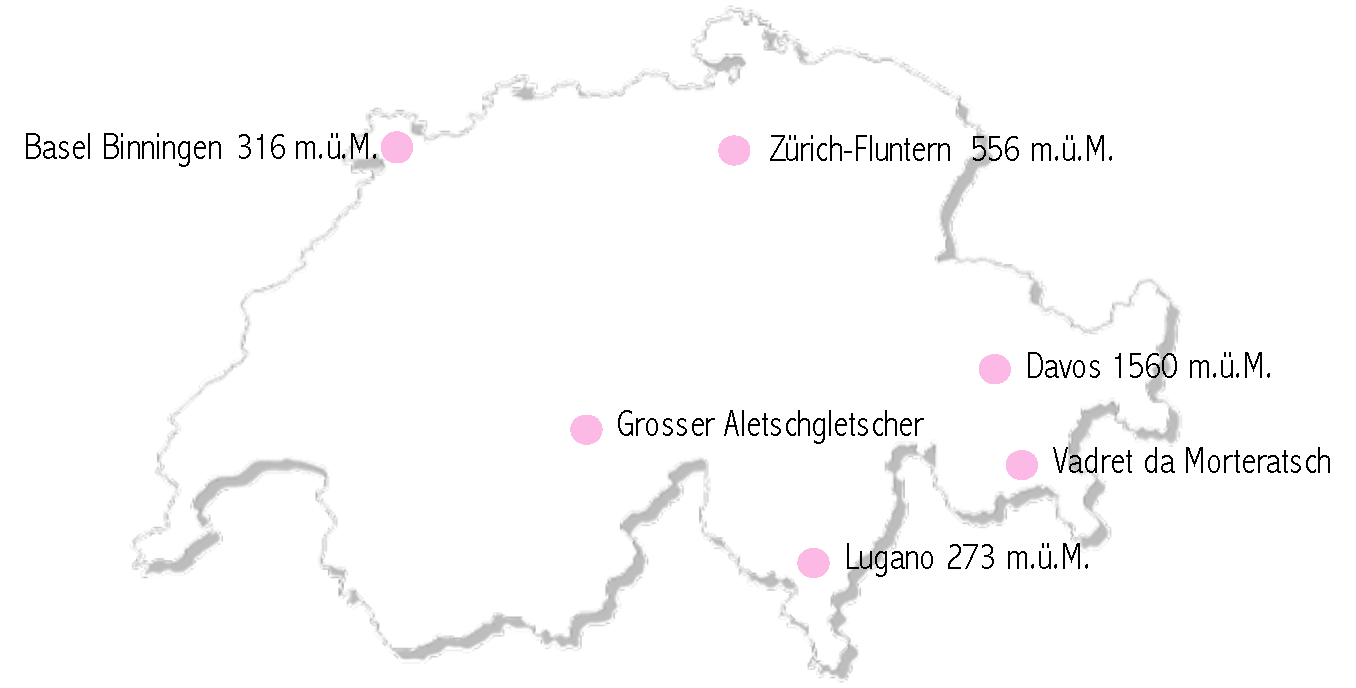
\includegraphics[width=0.8\textwidth]{extrem/Schweiz.pdf}
\caption{Gewählte Messpunkte in der Schweiz.}
\label{MesspunkteCH}
\end{figure}

Die Messreihen der Standorte Basel Binningen, Zürich-Fluntern, Lugano und Davos sind von MeteoSchweiz und sind öffentlich zugänglich. Die Daten sind bereits homogenisiert.
Die Messdaten der Gletscher werden vom Schweizerischen Gletschermessnetz
GLAMOS\footnote{%
Die Veränderungen der Schweizer Gletscher werden jährlich gemessen. Das Messnetz GLAMOS wird getragen durch die ETH Zürich und die Universitäten Fribourg und Zürich mit finanzieller Unterstützung durch das Bundesamt für Umwelt BAFU, MeteoSchweiz und SCNAT.} ebenfalls öffentlich zugänglich, zur Verfügung gestellt.


\subsection{Prüfung Messreihe}
Die Messreihen geben einen Einblick über die letzten 75 Jahre, nämlich von 1943--2017. Damit die Hypothese widerlegt wird und somit der Klimawandel nachgewiesen werden kann, müssen drei oder mehr extreme Ereignisse in den letzten 10 Jahren vorkommen (Abbildung \ref{TabExt}). Das Signifikanzniveau $\alpha = 5\%$ wird unterschritten \ref{SigniAlpha}) und die Hypothese widerlegt.
Die detaillierten Auswertungen der Messreihen und Gletscherdaten sind im Abschnitt~\ref{AuswertungKG} aufgeführt.


\section{Temperaturanstieg wegen Klimawandel?}
\rhead{Temperaturanstieg wegen Klimawandel?}
Die Jahresmitteltemperatur in der Schweiz ist seit 1864 rund $2^{\circ}$C gestiegen (Stand 2018, MeteoSchweiz). Der grösste Anstieg passierte in den letzten Jahrzehnten. Dennoch ist für die breite Bevölkerung ein Anstieg von $2^{\circ}$C schwierig nachzuvollziehen.
In den nachfolgenden Beispielen, wurden Klimaindikatoren gewählt, die jeder kennt, spürbar sind und beobachtet werden können.

\subsection{Jahresmitteltemperatur}
\index{Jahresmitteltemperatur}
Die Jahresmitteltemperatur ist wie folgt definiert.

\begin{definition}
Mittlere Jahrestemperatur in $^{\circ}$C.\footnote{%
Systematische Messungen an den Messstationen mehrmals pro Tag. Die gemittelten Tagestemperaturen pro Tag, ergeben die mittlere Jahrestemperatur.}
\end{definition}

Bei der Jahresmitteltemperatur ist das Ergebnis eindeutig (Abbildung \ref{JMittel}). Bei beiden Messpunkten, sowohl Lugano als auch Basel Binningen, wird der Hypothesentest widerlegt da die Alphagrenze deutlich unterschritten wird. Bei Basel Binningen kommen vier der extremsten Ereignisse in den letzten 10 Jahren vor. In Lugano sind es sogar deren fünf! Der Klimawandel ist ohne jeden Zweifel nachgewiesen.


\subsection{Sommertage}
\index{Sommertage}
Ein Sommertag ist wie folgt definiert.

\begin{definition}
Maximale Temperatur $\ge 25^{\circ}$C.
\end{definition}

Die Sommertage in Lugano waren in den letzten 10 Jahren nie extrem (Abbildung \ref{Sommertage}). Zu Beginn der Messungen in den 40er und 50er Jahren zeigen sich Extremwerte. Wohingegen Davos eine Häufung der Anzahl von Sommertagen in den letzten 10 Jahren zeigt. In den früheren Messjahren waren keine oder nur sehr wenige Sommertage vorhanden. In den letzten 10 Jahren ist die Anzahl der Sommertage aber immer weiter gestiegen und mit 5 Ereignissen eigentlich nahezu unmöglich. In Davos wird die Hypothese widerlegt und somit ein Wandel im Klima nachgewiesen.


\subsection{Tropennächte}
\index{Tropennächte}
Eine Tropennacht ist wie folgt definiert.

\begin{definition}
Minimale Temperatur $\ge 20^{\circ}$C.
\end{definition}

Sowohl in Lugano wie auch Basel Binningen sind in den letzten 10 Jahren eine extreme Anzahl von Tropennächten gemessen worden (Abbildung \ref{Tropennacht}). Mit vier Ereignissen pro Standort wird das Signifikanzniveau deutlich unterschritten, wie in den vorangegangenen Messreihen {\em Jahresmitteltemperatur} und {\em Sommertage} ist der Klimawandel real und nachgewiesen.


\subsection{Hitzetage}
\index{Hitzetage}
Ein Hitzetag ist wie folgt definiert.

\begin{definition}
Maximale Temperatur $\ge 30^{\circ}$C.
\end{definition}

Bei den Hitzetagen ist im Klima kein Wandel zu erkennen (Abbildung \ref{Hitzetage}). Weder in Zürich-Fluntern noch in Lugano wurden in den letzten Jahren extrem viele Hitzetage gemessen. Bei beiden Orten, waren Hitzetage zu Beginn der Messreihen in den 40er Jahren häufiger.


\subsection{Frosttage}
\index{Frosttage}
Ein Frosttag ist wie folgt definiert.

\begin{definition}
Minimale Temperatur $< 0^{\circ}$C.
\end{definition}

Wie bereits bei den Hitzetagen ist auch bei den Frosttagen weder in Basel Binningen noch in Lugano kein Wandel im Klima zu erkennen (Abbildung \ref{Frosttage}). Ebenso wurden die Extremen vermehrt zu Beginn der Messreihe gemessen.


\subsection{Eistage}
\index{Eistage}%
Ein Eistag ist wie folgt definiert.

\begin{definition}
Maximale Temperatur $< 0^{\circ}$C.
\end{definition}

Anhand der Anzahl Eistage in Zürich-Fluntern und Davos, kann kein Klimawandel festgestellt werden (Abbildung \ref{Eistage}). Weder in den oberen noch in den unteren Extremen. 


\section{Niederschlag und Klimawandel}
\rhead{Niederschlag und Klimawandel}
In den letzen Jahren nahmen die Niederschläge zu. Die Schadensumme der Hochwasserereignisse in der Schweiz beläuft sich durchschnittlich auf 300 Millionen Schweizer Franken pro Jahr. Vor allem im Jahr 2005 kam es zu extremen Hochwasserereignissen infolge starker Unwetter welche über die Schweiz zogen. Ausuferungen, Überschwemmungen und Schlammlawinen waren die Folgen heftigen Unwetter. Die Schadensumme belief sich auf 3 Milliarden Schweizer Franken. 


\subsection{Jahresniederschlag}
\index{Jahresniederschlag}%
Der Jahresniederschlag ist wie folgt definiert.

\begin{definition}
Jahresniederschlag in mm.
\end{definition}

Der Jahresniederschlag hat in den letzten Jahren zwar zugenommen, zeigt aber keine Häufung von extremen Ereignissen in den letzten 10 Jahren (Abbildung \ref{Jahresniederschlag}). Anhand des Jahresniederschlags kann man nicht auf den Klimawandel schliessen. Hier wäre es interessant eine Messereihe zu testen, welche die Anzahl Starkniederschläge pro Jahr aufzeigt.


\subsection{Neuschnee}
\index{Neuschnee}%
Die Neuschneemenge ist wie folgt definiert.

\begin{definition}
Neuschneemenge, Jahressumme der täglichen Aufzeichnung in cm.
\end{definition}

Ähnlich sieht es bei der Neuschneemenge aus (Abbildung \ref{Neuschnee}). In Davos ist kein Klimawandel festzustellen, weder in der oberen oder unteren Grenze. In Basel Binningen wurden in den letzten 10 Jahren keine extremen Neuschneemengen im oberen Grenzbereich verzeichnet, jedoch im unteren Bereich zeigt sich eine Änderung. Der Klimawandel ist festzustellen.
Hier wäre es ebenfalls spannend, die Fragestellung anzupassen und abzuändern in: Wie lange bleibt der Neuschnee liegen?


\section{Gletscherschwund?}
\rhead{Gletscherschwund?}
\index{Gletscherschwund}%
Bei den Gletscherdaten wurde der Zeitraum von 1881--2017 gewählt. Durch die höhere Anzahl an Messjahren, müssen die Wahrscheinlichkeitswerte neu berechnet werden. Die Berechnungen ergeben leicht veränderte Werte, es müssen aber ebenso 3 oder mehr extreme Ereignisse in den letzten 10 Jahren vorkommen um diese dem Klimawandel zuschreiben zu können.


\subsection{Grosser Aletschgletscher}
\index{Aletschgletscher}%
Der grosse Aletschgletscher schmilzt, wie man gut auf der (Abbildung \ref{Aletsch}) sehen kann. Jedoch zeigen die Messwerte der letzen 136 Jahren keinen extremen Schwund der Eismassen auf.
%
Anhand der Messdaten ist kein Klimawandel nachweisbar (Abbildung \ref{AletschTab}). Hier müsste allerdings die Messreihe hinterfragt werden. Die Messreihe zeigt nur die Längenänderung pro Jahr wieviel die Gletscherzunge schwindet und nicht die Volumenänderung der Eismasse. Der Gletscher könnte in der Länge nur wenig schwinden, würde aber im selben Jahr sehr viel an Volumen verlieren, wäre dies dennoch nicht in der Messreihe ersichtlich.


\subsection{Vadret da Morteratsch}
\index{Morteratschgletscher}
Beim Morteratschgletscher sieht es anders aus. Die Längenänderung in den letzten 10 Jahren ist massiv (Abbildung \ref{Morteratschtab}). Hier kann aufgrund der extremen Längenänderung auf den Klimawandel geschlossen werden. Dies ist auch deutlich in der (Abbildung \ref{Morteratsch}) ersichtlich. Speziell in diesem Fall wäre es spannend herauszufinden, ob die Abnahme des Eisvolumens ebenso auf den Klimawandel schliessen lässt oder nicht.


\section{Ist der Klimawandel in der Schweiz real?}
\rhead{Ist der Klimawandel in der Schweiz real?}
Die in diesem Kapitel beschriebene Methode liefert schnell und einfach ein Ergebnis ob eine Veränderung in einer Klimamessreihe dem Klimawandel zugeschrieben werden kann oder ob es sich um eine zufällige Häufung von extremen Ereignissen handelt. Aus den analysierten Klimaindikatoren ist der Klimawandel nicht immer eindeutig hervorgegangen (Abbildung \ref{AuswertungK}). 

Dennoch lässt sich die Frage, ob der Klimawandel in der Schweiz real ist, deutlich mit {\em Ja} beantworten. Vor allem die Indikatoren rund um die Temperatur zeigen einen deutlichen Wandel. Besonders die Messreihen der {\em Jahresmitteltemperatur}, {\em Tropennächte} und die {\em Sommertage}, weisen eine starke Veränderung im Vergleich zur Vergangenheit auf. Wohingegen bei den Niederschlägen und dem Aletschgletscher (Abbildung \ref{AuswertungG}) kein Klimawandel festgestellt werden konnte. Mit den Vorschlägen zur Untersuchung von weiteren und anders formulierten Messreihen, könnte ein Wandel eventuell auch noch bei anderen Klimaindikatoren und Messreihen aufgezeigt werden.


\begin{table}
\centering
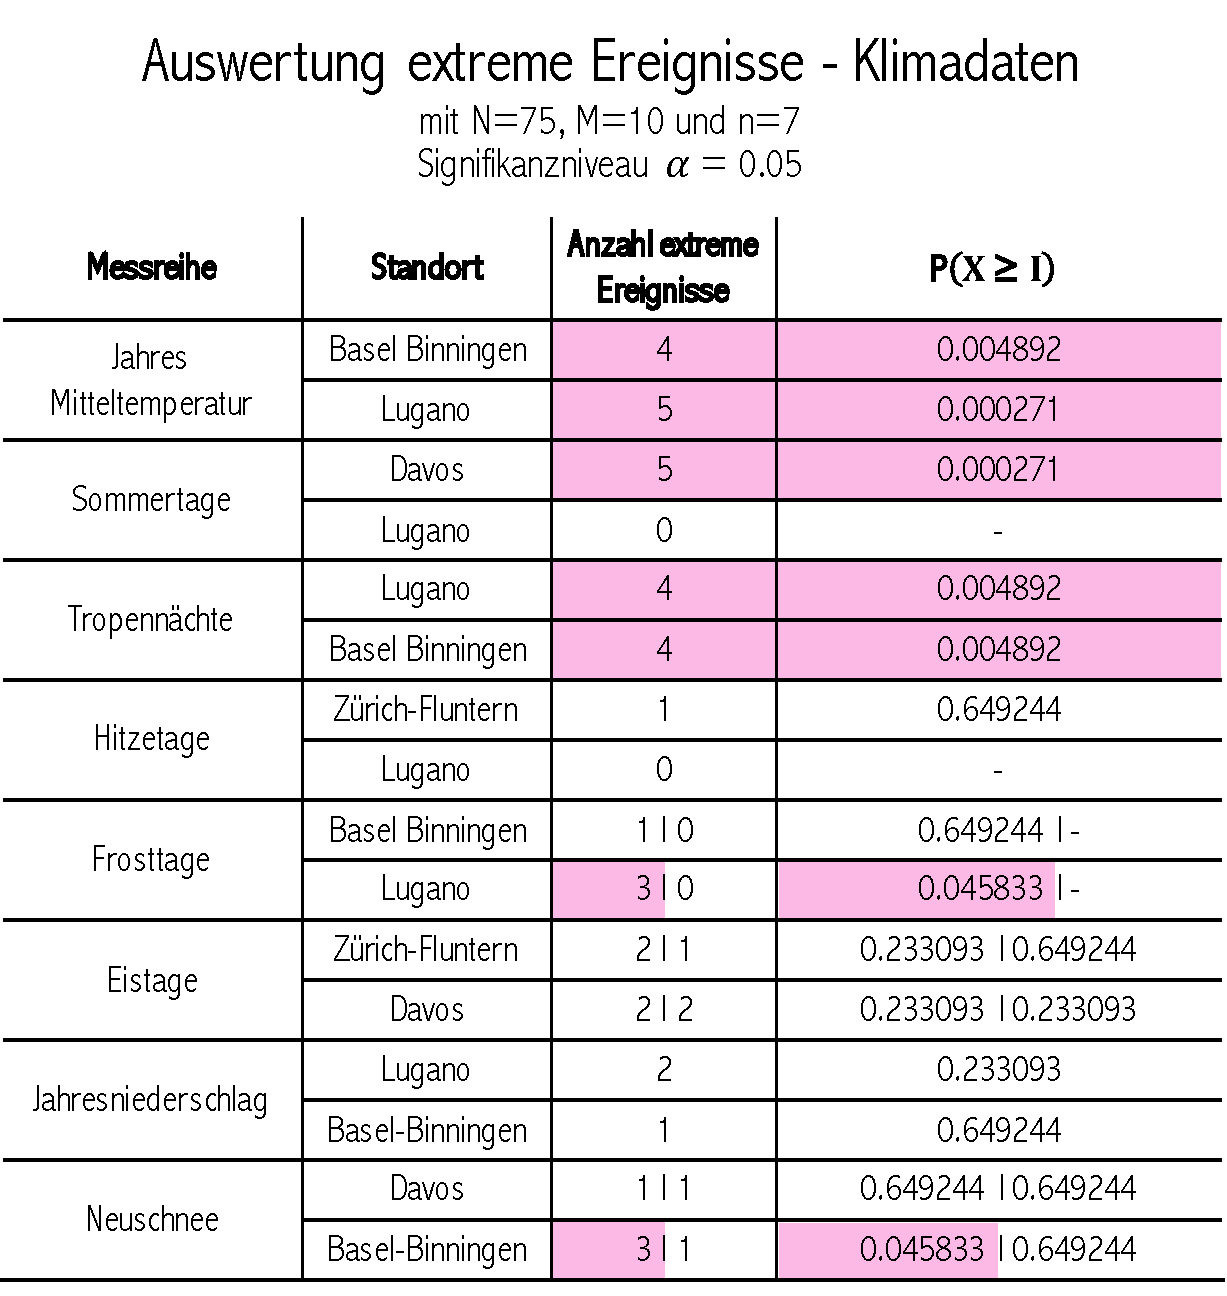
\includegraphics[width=0.7\textwidth]{extrem/AuswertungK.pdf}
\caption{Die Auswertung der Klimadaten schafft einen Überblick, welche Klimaindikatoren vom Klimawandel betroffen sind und welche nicht. Rosa markiert sind jene, welche das Signifikanzniveau $\alpha=0.05$ unterschreiten. Die Häufung jener extremen Ereignisse (in den letzten 10 Jahren), ist dem Klimawandel zuzuschreiben.}
\label{AuswertungK}
\end{table}


\begin{table}
\centering
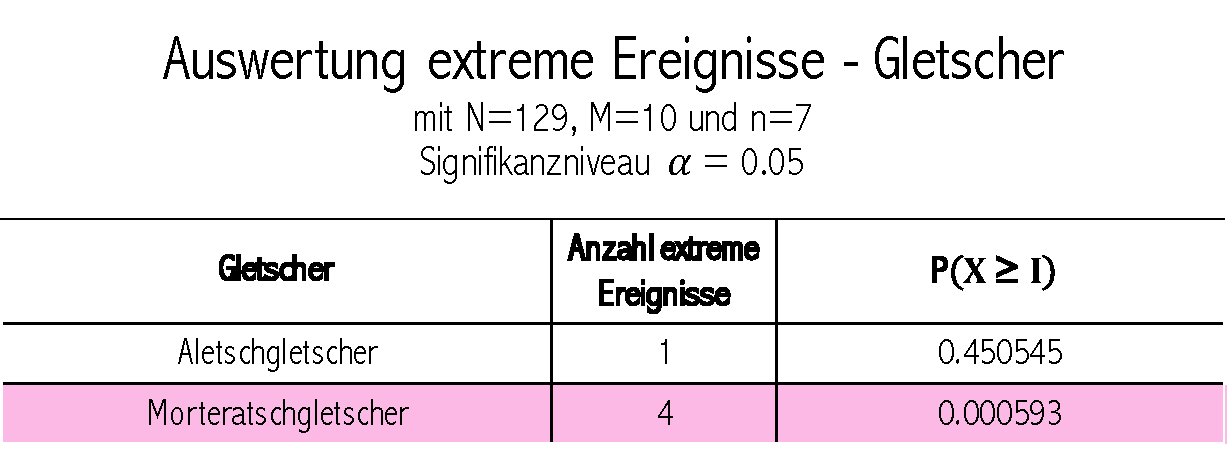
\includegraphics[width=0.7\textwidth]{extrem/AuswertungG.pdf}
\caption{Die Auswertung der Gletscherdaten schafft ebenso einen Überblick über die beiden Gletscher ob diese vom Klimawandel betroffen sind oder nicht.}
\label{AuswertungG}
\end{table}

Mit dieser Berechnungsweise lässt es sich ohne Vorurteile und Einflüsse neutral bewerten, ob der Klimawandel vorhanden ist oder nicht. Aufgrund der Tatsache, dass von acht getesteten Klimaindikatoren, fünf die Hypothese widerlegen, kann davon ausgegangen werden, dass der Klimawandel real ist. Das Klima ändert sich und ob dies gut oder schlecht für die Menschheit ist, wird sich in der Zukunft zeigen. Feststeht, dass die Erde auch dieses extreme Ereignis wie den Klimawandel überstehen wird --- mit oder ohne uns, das liegt in unseren Händen.


\section{Ist der Klimawandel nur ein grosser Zufall?}
\rhead{Ist der Klimawandel nur ein grosser Zufall?}
Als Jim Inhofe\footnote{%
\index{Inhofe, Jim}%
James \glqq Jim\grqq{} Inhofe, ist ein US-amerikanischer Politiker (Republikanische Partei) und Senator für den Bundesstaat Oklahoma. Seit Januar 2015 ist er Vorsitzender des Ausschusses für Umwelt und öffentliche Bauten. Er vergleicht Menschen, die an die globale Erwärmung und somit den Klimawandel glauben, mit Nazis und die US-Umweltbehörde EPA (United States Environmental Protection Agency) mit der Gestapo.} im Februar 2015 in die Senatssitzung einen Schneeball mitbrachte, wollte er mit der Existenz des Schnees beweisen, dass es keine globale Erwärmung gibt. Zudem soll der Schneeball Beweis dafür sein, dass die Rekordtemperaturen aus dem Jahr 2014 ebenfalls nichts mit dem Klimawandel zu tun haben. Er unterstrich seine Aussagen und Begründungen mit einem Bibelvers aus dem 1. Buch Mose.

\begin{quote} 
Solange die Erde steht, soll nicht aufhören Saat und Ernte, Frost und Hitze, Sommer und Winter, Tag und Nacht.
\end{quote}

Frost und Hitze, Sommer und Winter --- dies soll nochmals beweisen, dass es keinen von Menschenhand gemachten Klimawandel gibt.
Ein Klimaskeptiker würde über unsere  Auswertungen denn Kopf schütteln und sagen: Das ist doch alles nur Zufall. Doch ist es das wirklich?

Sehen wir uns die statistischen Auswertungen rein mathematisch an, wird das Signifikanzniveau $\alpha$ = 5\% deutlich unterschritten. Die Nullhypothese ist sogar dann widerlegt, wenn man das Signifikanzniveau auf $\alpha$ = 1\% senken würde (Jahresmitteltemperatur, Sommertage, Tropennächte). Wäre der Klimawandel nicht vom Menschen wesentlich mit verursacht, wäre die Wahrscheinlichkeit so viele extreme Ereignisse in den letzten 10 Jahren vorzufinden, nur 5\%. Sehr unwahrscheinlich, dass dies bei so vielen Klimaindikatoren eingetroffen ist. Mathematisch gesehen muss eine Klimaänderung stattfinden.

Betrachten wir erneut die Aussage von Jim Inhofe: Die Klimaforscher behaupten keineswegs, dass es mit der globalen Erderwärmung keinen Schnee mehr gibt. Dies ist auch in der nachfolgenden Auswertung ersichtlich. Obwohl die Jahresmitteltemperatur das Signifikanzniveau deutlich unterschreitet und damit wärmere Temperaturen in einem Jahr erreicht werden, gibt es immer noch Schnee. 

\subsection{Auswertung und Erklärung der Klimadaten}
Wie bereits oben erwähnt, ist die Auswertung bei der Jahresmitteltemperatur sehr deutlich.  Dies deckt sich auch mit dem im Kapitel \ref{skript:section:budyko} erklärten Treibhauseffekt. Das CO$_2$ welches {\em en masse} von der Menschheit in die Atmosphäre gepumpt wird, ist der Hauptgrund für den globalen Temperaturanstieg.

Bei den Sommertagen wurde das Signifikanzniveau in Davos unterschritten, wohingegen Lugano keine extremen Ereignisse in den letzten 10 Jahren zeigt. 

Bei den Tropennächten wurde an beiden Standorten der Klimawandel festgestellt. Aufgrund der fortlaufenden Veränderung des Klimas kann es durchaus vorkommen, dass die extremen Ereignisse in den nächsten Jahren nicht mehr vorkommen. Mit dem globalen Temperaturanstieg befindet sich mehr Wasser und Energie in der Atmosphäre. Dies kann vermehrt zu Gewittern am Abend führen. Die Temperatur wird durch das Gewitter und einen allfälligen Regenschauer sinken und dadurch keine Tropennacht verzeichnet. Der Klimaindikator {\em Tropenacht} reagiert sehr empfindlich auf Änderungen.
%
Ähnlich sieht es bei den Hitzetagen aus. Im Moment zeigen sich in den letzten 10 Jahren keine nennenswerten Häufungen von Klimaextreme, trotzdem ist ein Aufwärtstrend zu erkennen. In den letzten Jahren wurden vermehrt Hitzetage registriert als vor der Jahrtausendwende. Mit dem weiteren Anstieg der Jahresmitteltemperatur ist es durchaus denkbar, in ein paar Jahren vermehrt extrem viele Hitzetage in der Messreihe zu verzeichnen.

Die Frost- und Eistage zeigen im Moment noch keine verwertbaren Anzeichen des Klimawandels. Ähnlich wie bei den Hitzetagen ist dennoch ein Trend zu erkennen. Es wurden deutlich weniger Frost- bzw. Eistage seit der Jahrtausendwende verzeichnet. Bei beiden Messstandorten Zürich-Fluntern wie auch Davos fehlt nur noch ein extremes Ereignis und der Klimawandel wird nachweisbar sein. Aufgrund des Abwärtstrends in den Frost- und Eistagen werden diese Klimaindikatoren ebenfalls als empfindlich eingestuft.

Über die Messjahre ist die Summe des Jahresniederschlags relativ konstant geblieben. Hier müsste untersucht werden, ob in den Starkniederschlägen oder jenen im Winter eine Änderung zu verzeichnen ist. Gemäss MeteoSchweiz wird ein höherer mittlerer Winterniederschlag verzeichnet (ausgenommen Südalpen und Teile des Kantons Graubünden). Zudem gibt es deutliche Hinweise, dass sich die Starkniederschläge verändern: Diese kommen häufiger und stärker (Tagessummen) vor, seit den Aufzeichnungen im Jahr 1901. Der Jahresniederschlag ist daher ein gutes Beispiel dafür, dass der Klimawandel sich nicht immer direkt auf eine Statistik auswirkt. Betrachtet man nur den Jahresniederschlag, sind keine Trends oder grosse Häufungen zu verzeichnen. Sieht man sich aber die Verteilung der Niederschläge an und deren Stärke, ist ein Wandel festzustellen.

Die gefallene Neuschneemenge ist in Basel Binningen in den letzten 10 Jahren gesunken. Ein Klimawandel wurde in der unteren extremen Grenze verzeichnet. Vergleicht man dies mit der Aussage von MeteoSchweiz, dass in den letzten Jahren vor allem in den tieferen Lagen weniger Schnee verzeichnet worden ist, trifft dies zu, den beispielsweise Davos zeigt keinen Wandel auf. Mit der steigenden Jahresmitteltemperatur erwärmt sich auch die Erdoberfläche. Würde man die Fragestellung anpassen in: Wie lange bleibt der Schnee liegen? Würde man den Aspekt der globalen Erwärmung zusätzlich berücksichtigen und den Wandel erkennen.


\subsection{Auswertung und Erklärung der Gletscher}
Mit dem Aletsch\footnote{%
Der Aletschgletscher ist 23 Kilometer lang, 80 Quadratkilometer gross und 27 Milliarden Tonnen schwer. Sein Ursprung liegt auf 4000 m.ü.M. in der Jungfrau Region.}
- und Morteratschgletscher\footnote{%
Der Morteratschgletscher (Vadret da Morteratsch) ist 6.4 Kilometer lang, 15.3 Quadratkilometer gross und hat ein Volumen von rund 1.2 Kubikkilometer Eis.}
verliert nicht nur der längste Gletscher der Schweizer Alpen, sondern auch der voluminöseste Gletscher Jahr für Jahr an Länge. Beim Morteratschgletscher ist der Klimawandel deutlich zu erkennen. Mit 4 extremen Ereignissen in den letzten 10 Jahren ist das Signifikanzniveau unterschritten. Aufgrund der Statistik lässt sich beim Aletschgletscher kein Klimawandel erkennen, dennoch schmilzt er. Ein Grund für sein langsameres Schmelzen und damit weniger extreme Ereignisse, ist die Eisdecke. Am Konkordiaplatz beträgt diese 900 Meter, im Süden nimmt die Mächtigkeit ab und die Dicke des Eises liegt noch bei 150 Meter. Im Vergleich: Die durchschnittliche Eisdecke beim Morteratschgletscher ist mit 75 Metern Dicke deutlich weniger massiv. 
Würde die Fragestellung und somit die statistischen Messwerte die Änderung der Eisdecke oder Volumenänderung angeben, wäre bei beiden Gletschern vermutlich ein Wandel zu erkennen. Beim Aletschgletscher hat die Eisdecke seit 1850 zum Teil um über 100 Meter abgenommen. Vor allem die Bergführer merken den Wandel jeden Tag. Wege und Plätze, welche sie jahrzehntelang benutzen und besuchten, sind nicht mehr vorhanden oder nicht mehr passierbar. Die Eisdecke ist unwiderruflich weggeschmolzen.

Ein weiteres Indiz ist die Häufung von Gletscherfunden. Am 19. September 1991 wurde auf 3208m Höhe, am Tisenjoch in den Ötztaler Alpen (Österreich/Italien), die Gletschermumie\footnote{%
Eine Gletschermumie ist eine Leiche, welche sich seit ihrem Tod permanent unter Frost befindet. Der tote Körper wird an einem sehr kalten Ort gleichmässig eingefroren.}
Ötzi\footnote{%
Ötzi ist die international bekannteste Gletschermumie überhaupt. Sie stammt aus der späten Jungsteinzeit (Kupfersteinzeit). Der Todeszeitpunkt des Mannes wurde zwischen 3359 und 3105 v. Chr. datiert und mithilfe Radiokohlenstoffdatierung festgestellt. Die Mumie ist somit ca. 5250 Jahre alt.}
gefunden. Der Mann lag etwa 5200 Jahre unter dem Eis begraben bis man ihn fand. Seit die Gefrierschränke der Urzeit schmelzen, kommen weltweit archäologische Funde zum Vorschein, wie Ötzi 1991. Wenn wir nichts ändern und den Klimawandel stoppen, wer weiss was das Eis in den nächsten Jahren noch preisgibt?


\subsection{Was kann die Menschheit aktiv gegen den Klimawandel tun?}
Der Klimawandel ist real. Klimaskeptiker und -verneiner belügen sich selbst und verschliessen die Augen vor der Realität. Die globale Erderwärmung ist auch nicht {\em made in china} (Abbildung \ref{DTrump}) wie Donald Trump kurz nach seiner Wahl zum Präsidenten der Vereinigten Staaten von Amerika (2016) behauptete.

\begin{figure}
\centering
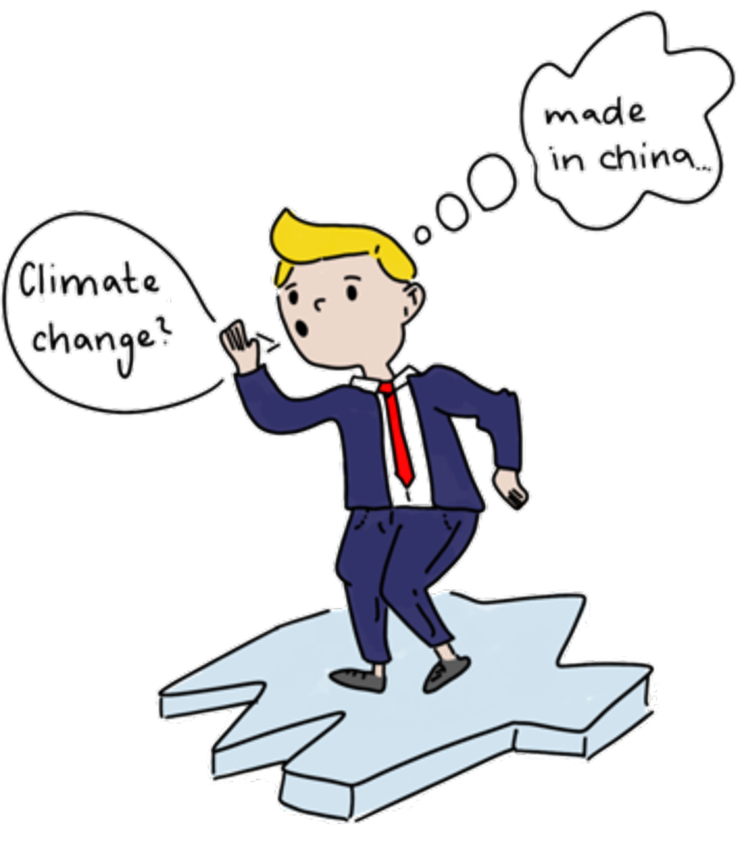
\includegraphics[width=0.4\textwidth]{extrem/Trump.pdf}
\caption{Das Konzept der globalen Erwärmung wurde von und für die Chinesen geschaffen, um die Wettbewerbsfähigkeit der US-Wirtschaft zu beschädigen. --- Donald Trump (2017)}
\label{DTrump}
\end{figure}

Der massive Ausstoss von Abgasen weltweit führt zur Erderwärmung
und steht damit in direktem Zusammenhang mit dem Klimawandel. Gelingt
es uns nicht, den Anstieg der globalen Durchschnittstemperatur
deutlich zu reduzieren und die Erwärmung unter $2^{\circ}$C zu
bleiben, dürfte der Klimawandel nicht mehr zu stoppen sein.
Fossile Brennstoffe werden in den nächsten Jahren ausgedient haben,
da sie nicht endlich sind und auch nicht mehr zeitgemäss sein werden.
Durch die Nutzung von Sonnen-, Wind- und Wasserenergie, durch
Biomasse und Geothermie entstehen kaum schädliche Emissionen und
der Treibhauseffekt wird nicht noch mehr gefördert.
Die Zukunft gehört den erneuerbaren Energien, die sich selber
regenerieren und nahezu unendlich sind. Die Einsicht etwas gegen
den Klimawandel zu tun muss weltweit geschehen damit das Ökosystem
der Erde nicht unwiderruflich zerstört wird.


\section{Auswertung der Klima- und Gletscherdaten} \label{AuswertungKG}
\rhead{Auswertung der Klima- und Gletscherdaten}
Nachfolgend aufgeführt sind die Auswertungen der Klima- und
Gletscherdaten.
Hier eine kurze Übersicht wie die Auswertungen der Klimadiagramme
gelesen werden müssen.
\begin{center}
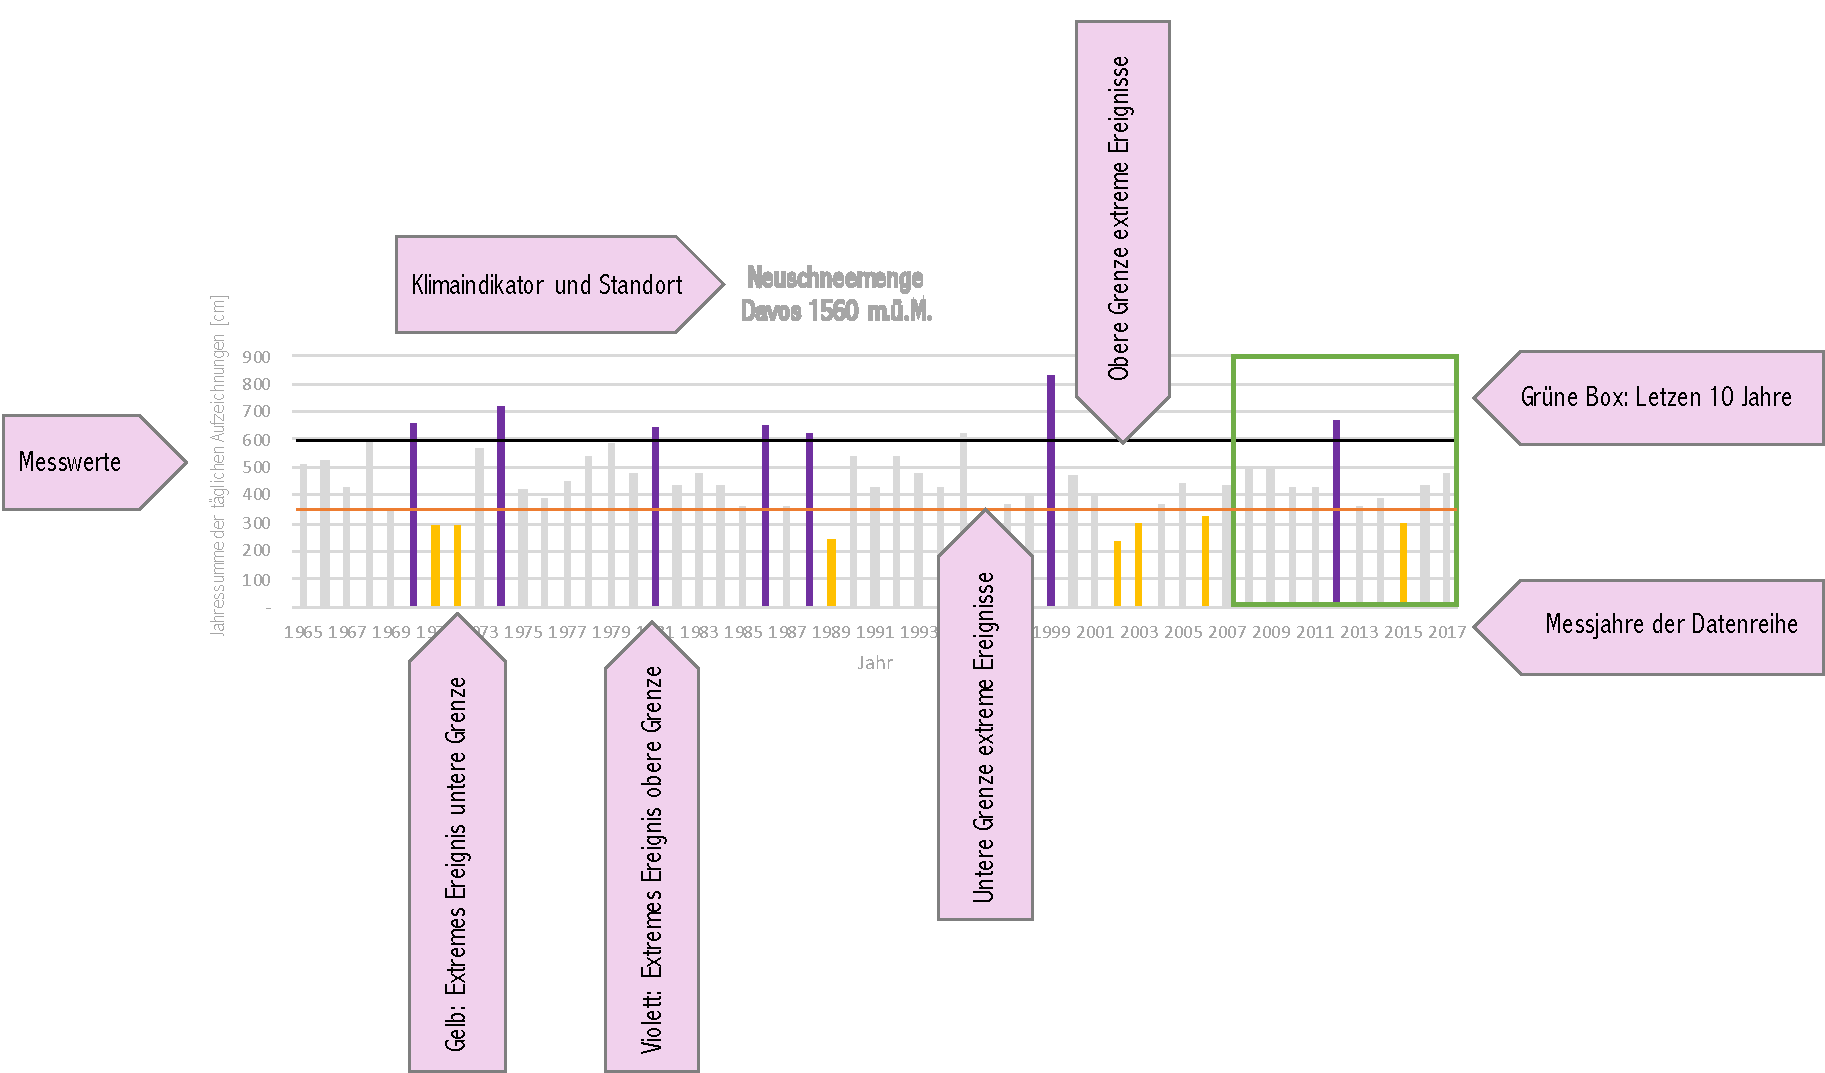
\includegraphics[width=1.0\textwidth]{extrem/Klimadiagrammlesen.pdf}
\end{center}
Zu beachten ist, dass nicht in allen Diagrammen
eine obere- und untere Grenze der Messwerte vorhanden ist. Rosafarbige
Balken bedeuten Messwerte im normalen Bereich, also keine Extremas.
%
%In der Tabelle
%\ref{Tabuebersicht} werden die verwendeten Werte der Variablen aufgezeigt.
%
%\begin{figure}
%\centering
%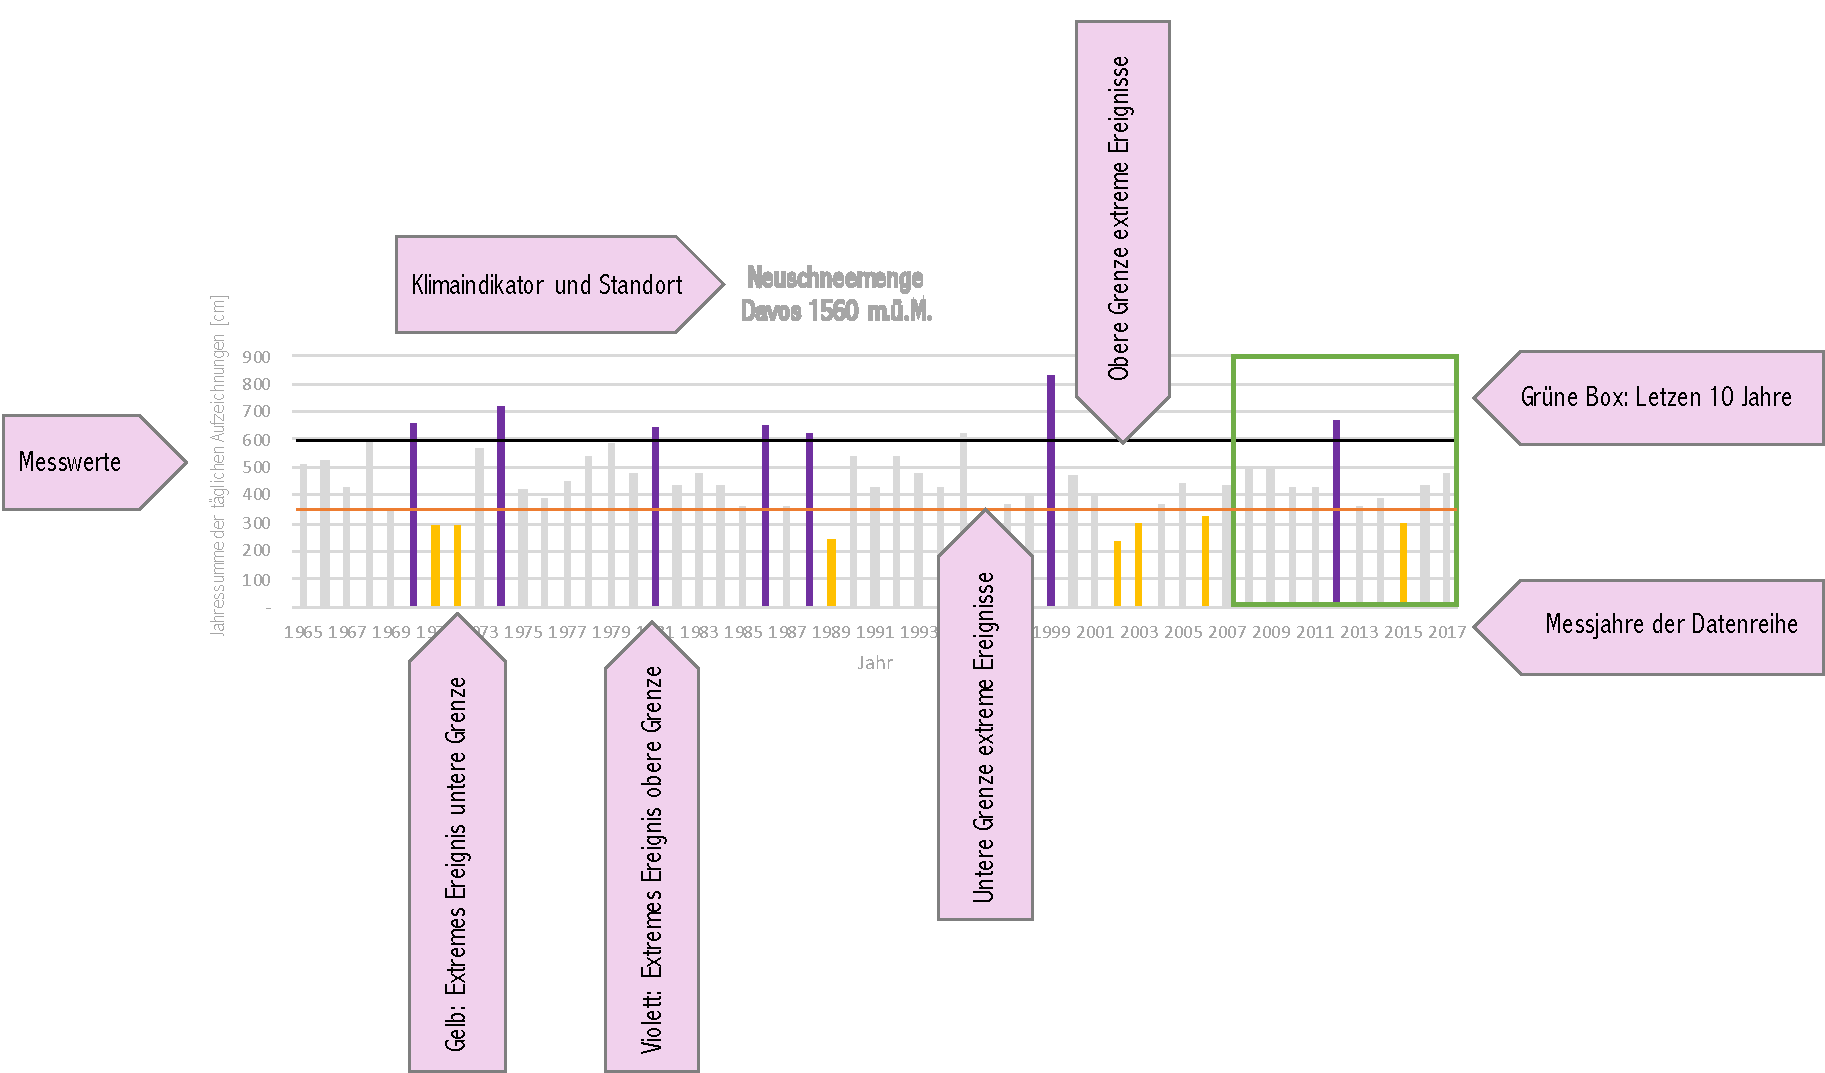
\includegraphics[width=1.0\textwidth]{extrem/Klimadiagrammlesen.pdf}
%\caption{Eine kurze Übersicht wie die Auswertungen der Klimadiagramme
%gelesen werden müssen. Zu beachten ist, dass nicht in allen Diagrammen
%eine obere- und untere Grenze der Messwerte vorhanden ist. Rosafarbige
%Balken bedeuten Messwerte im normalen Bereich, also keine Extremas.}
%\label{KlimaDia}
%\end{figure}
%
%\begin{table}
%\centering
%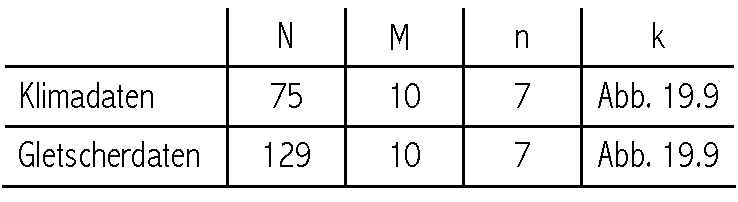
\includegraphics[width=0.5\textwidth]{extrem/Tabuebersicht.pdf}
Die verwendeten Werte der Variablen $N$, $M$, $n$ und $k$ sind
\begin{center}
\begin{tabular}{l|>{$}c<{$}|>{$}c<{$}|>{$}c<{$}|l}
              &N  & M&n&$k$\\
\hline
Klimadaten    & 75&10&7&Abbildung~\ref{TabExt}\\
Gletscherdaten&129&10&7&Abbildung~\ref{TabExt}\\
\end{tabular}
\end{center}
%\caption{Übersicht der verwendeten Werte der Variablen $N$, $M$, $n$ und $k$.}
%\label{Tabuebersicht}
%\end{table}


\begin{figure}
\centering
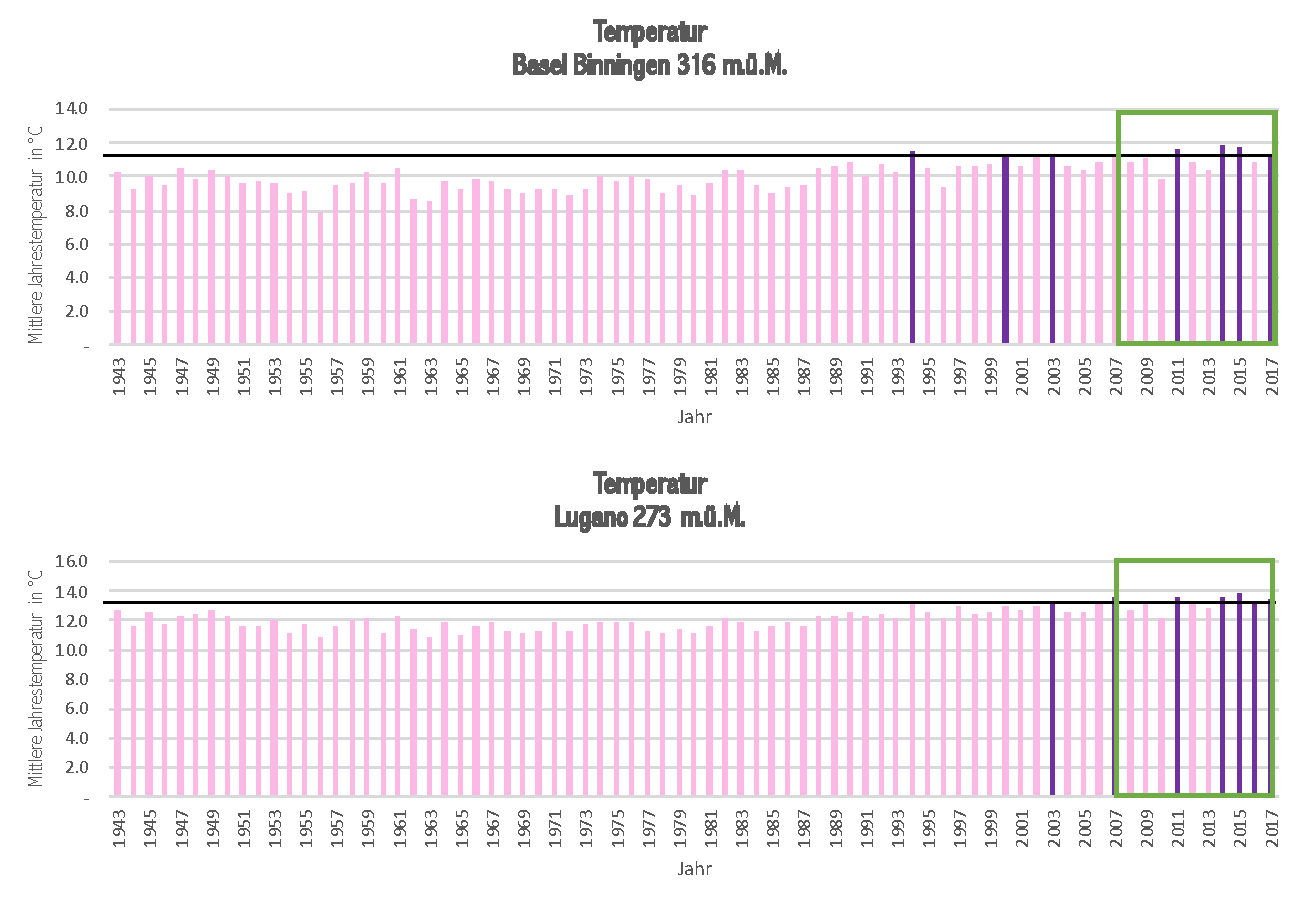
\includegraphics[width=0.8\textwidth]{extrem/JahresMittel.pdf}
\caption{Die Jahresmitteltemperatur der beiden Standorte Basel Binningen und Lugano. Bei beiden Standorten wird das Signifikanzniveau deutlich unterschritten und der Klimawandel ist nachgewiesen.}
\label{JMittel}
\end{figure}


\begin{figure}
\centering
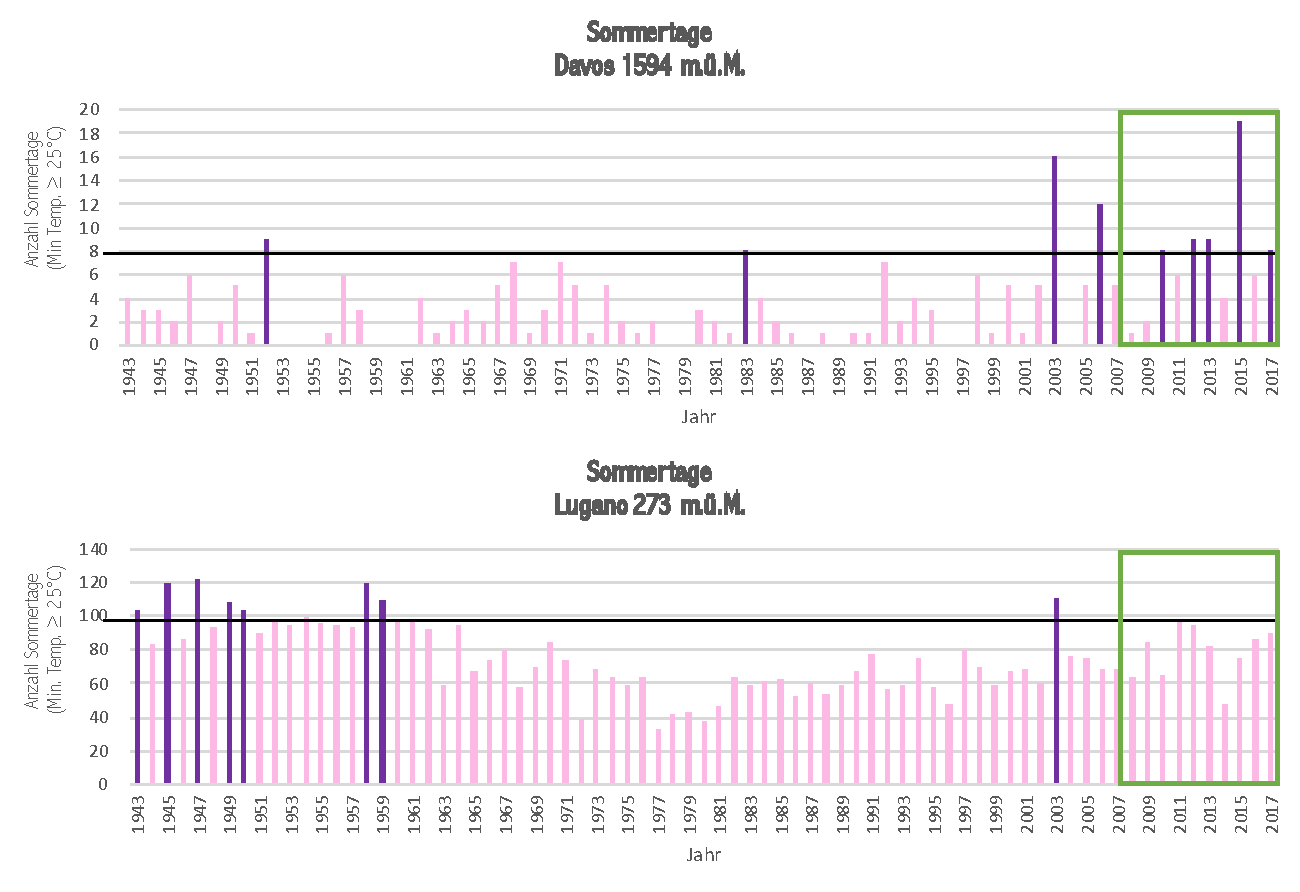
\includegraphics[width=0.8\textwidth]{extrem/Sommertage.pdf}
\caption{Die Anzahl Sommertage im Verlauf der Messreihe an den Standorten Davos und Lugano. Beim Standort Davos kann der Klimawandel nachgewiesen werden, da 5 extreme Ereignisse in den letzten 10 Jahren stattgefunden haben.}
\label{Sommertage}
\end{figure}


\begin{figure}
\centering
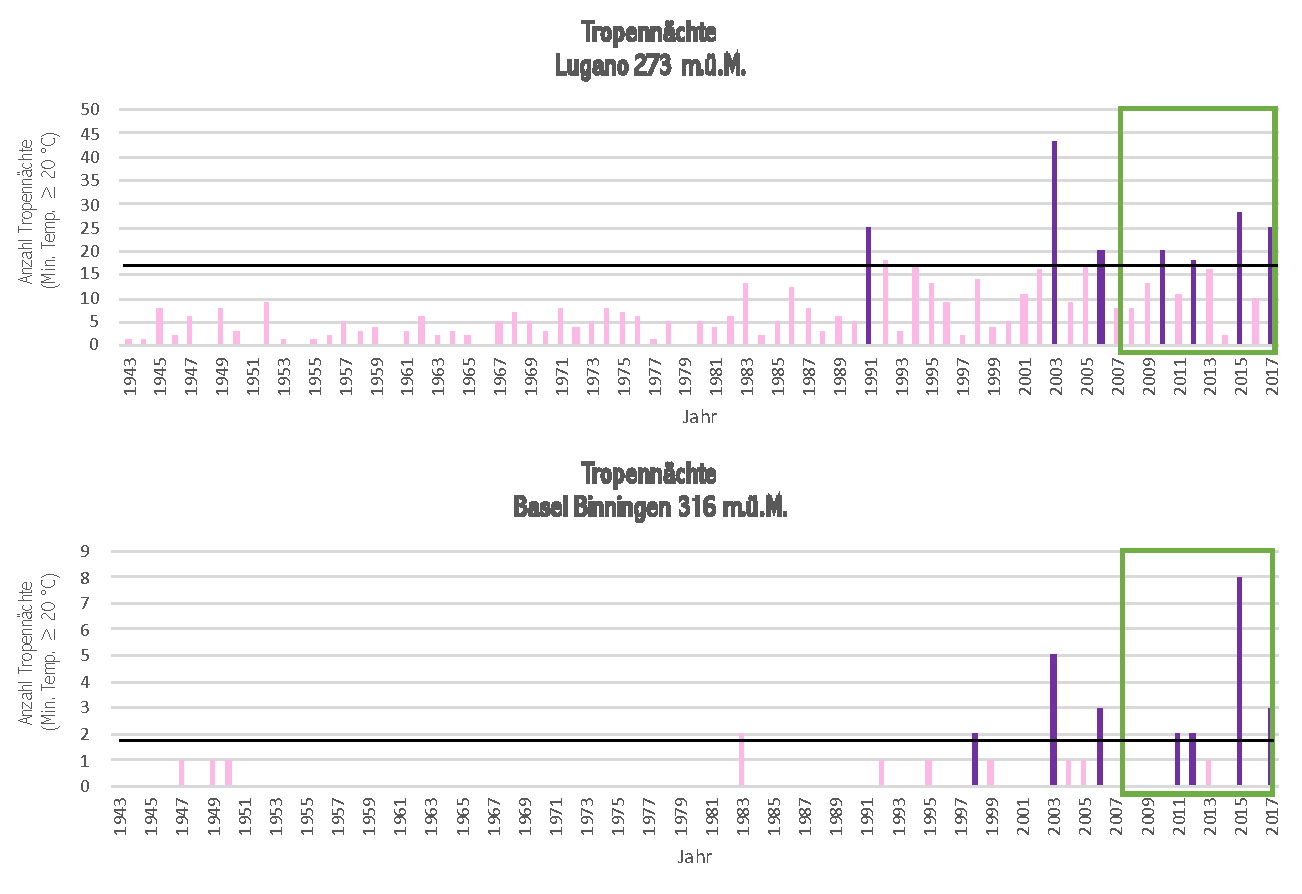
\includegraphics[width=0.8\textwidth]{extrem/Tropennacht.pdf}
\caption{Die Anzahl Tropennächte an den Standorten Basel Binningen und Lugano in den vergangenen Jahren. Bei beiden Standorten wird der Klimawandel nachgewiesen.}
\label{Tropennacht}
\end{figure}


\begin{figure}
\centering
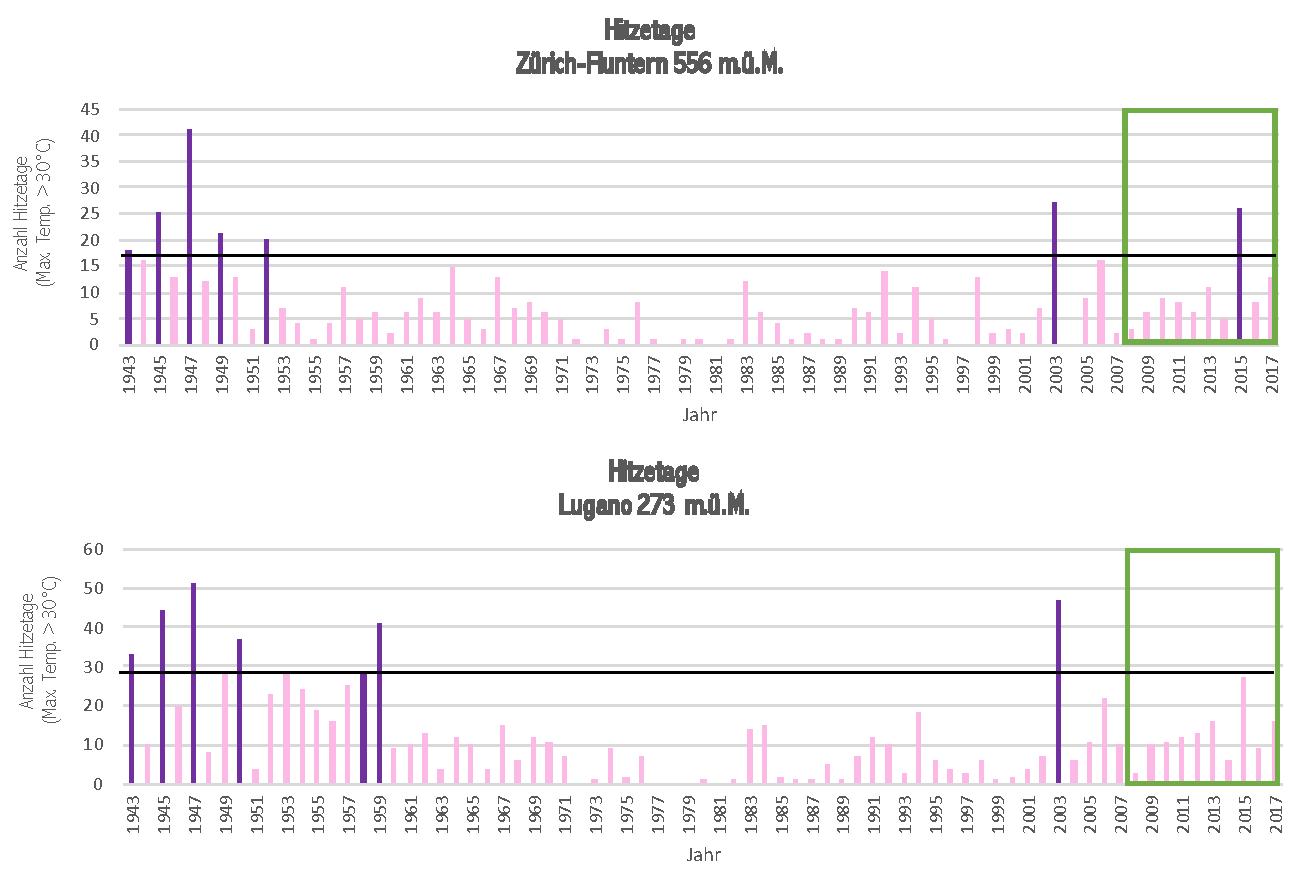
\includegraphics[width=0.8\textwidth]{extrem/Hitzetage.pdf}
\caption{Die Anzahl Hitzetage in der Messreihe an den Standorten Lugano und Zürich-Fluntern. Keine der beiden Standorte weisst anhand der Auswertung einen Klimawandel auf.}
\label{Hitzetage}
\end{figure}


\begin{figure}
\centering
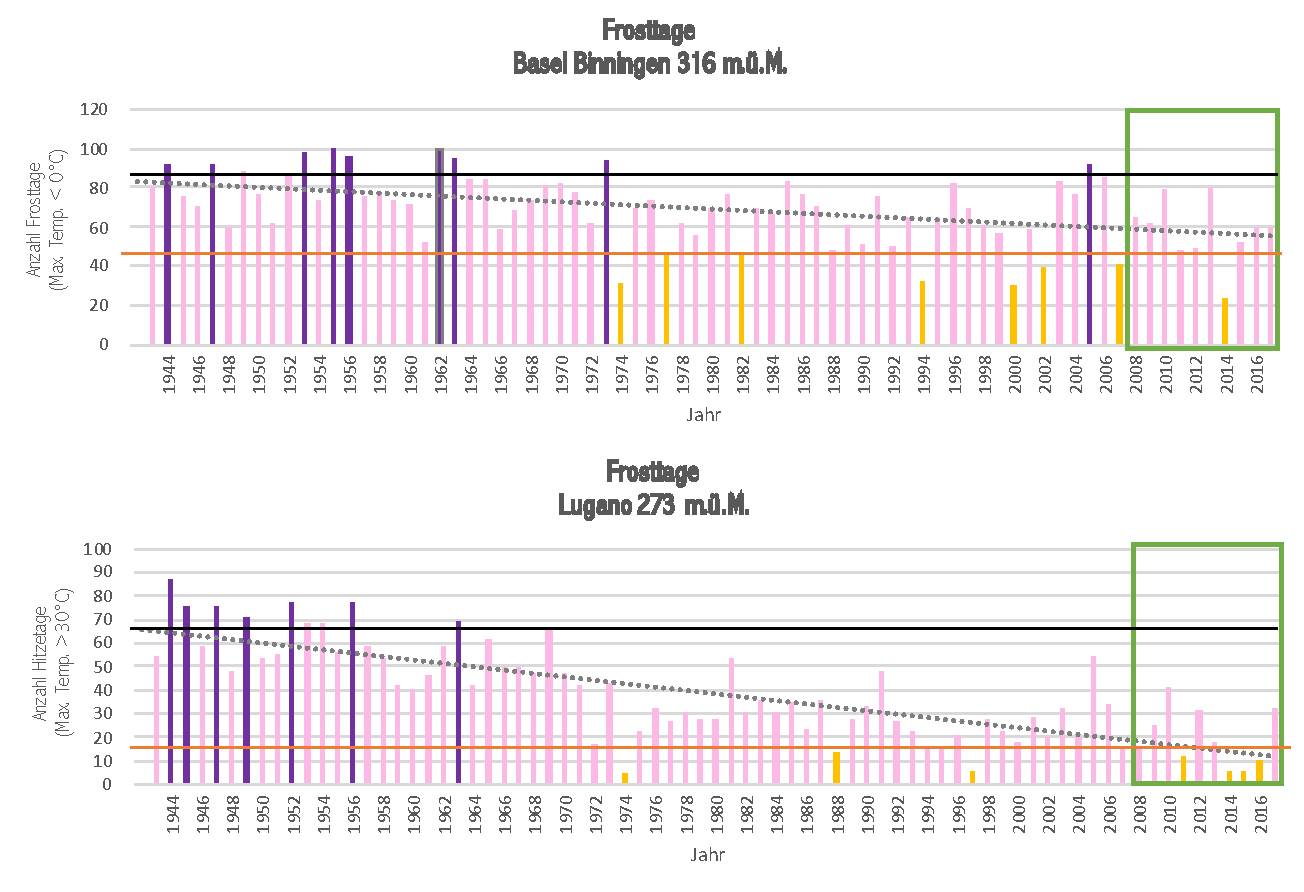
\includegraphics[width=0.8\textwidth]{extrem/Frosttage.pdf}
\caption{Die Anzahl Frosttage an den Standorten Lugano und Basel Binningen mit den oberen (violett) und unteren (gelb) Extremen Messwerten. Der Standort Lugano weisst mit den extrem wenigen Frosttagen einen Wandel im Klima auf.}
\label{Frosttage}
\end{figure}


\begin{figure}
\centering
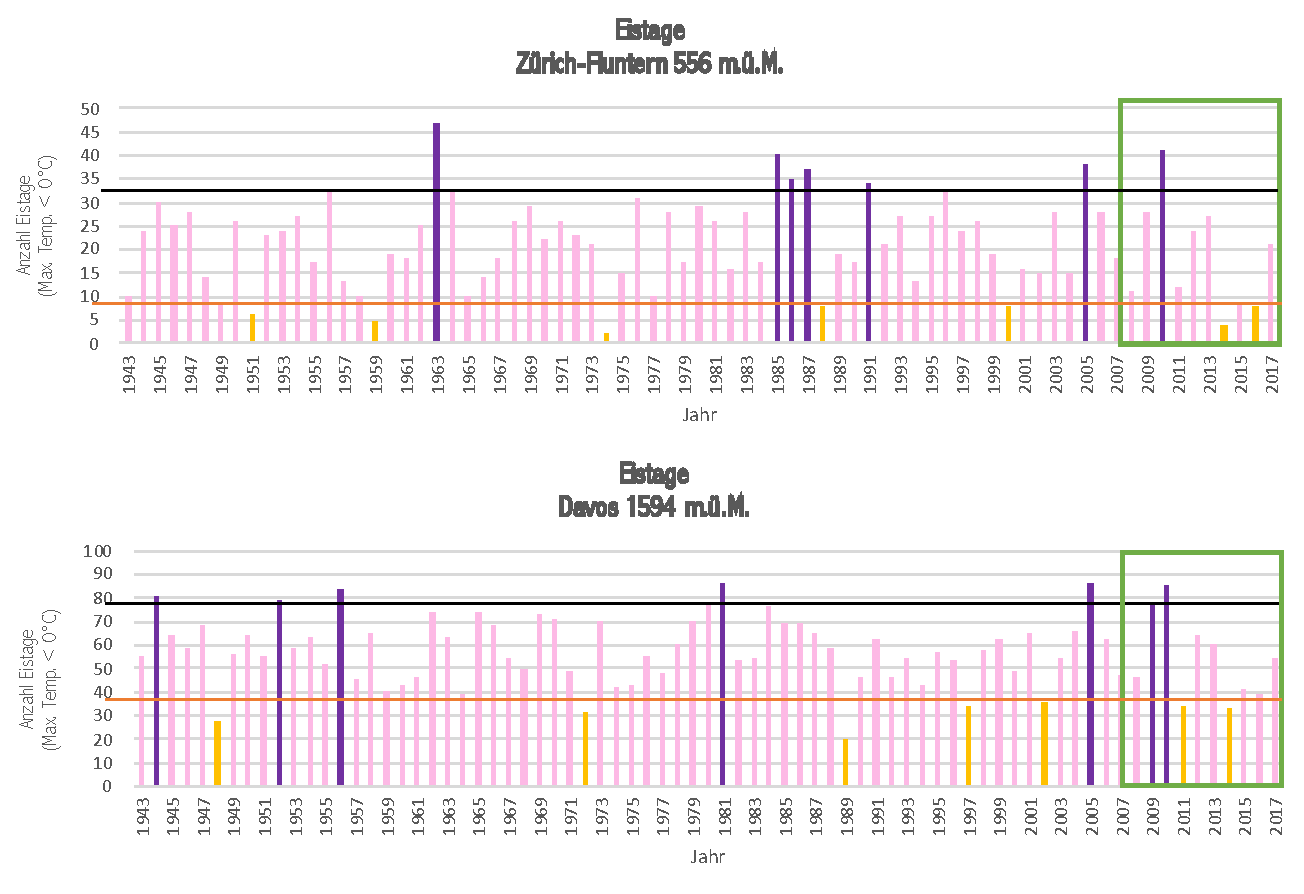
\includegraphics[width=0.8\textwidth]{extrem/Eistage.pdf}
\caption{Die Anzahl Eistage an den Standorten Zürich-Fluntern und Davos. Weder die obere (violett) noch die untere (gelb) extremen Ereignisse sind dem Klimawandel zuzuschreiben.}
\label{Eistage}
\end{figure}


\begin{figure}
\centering
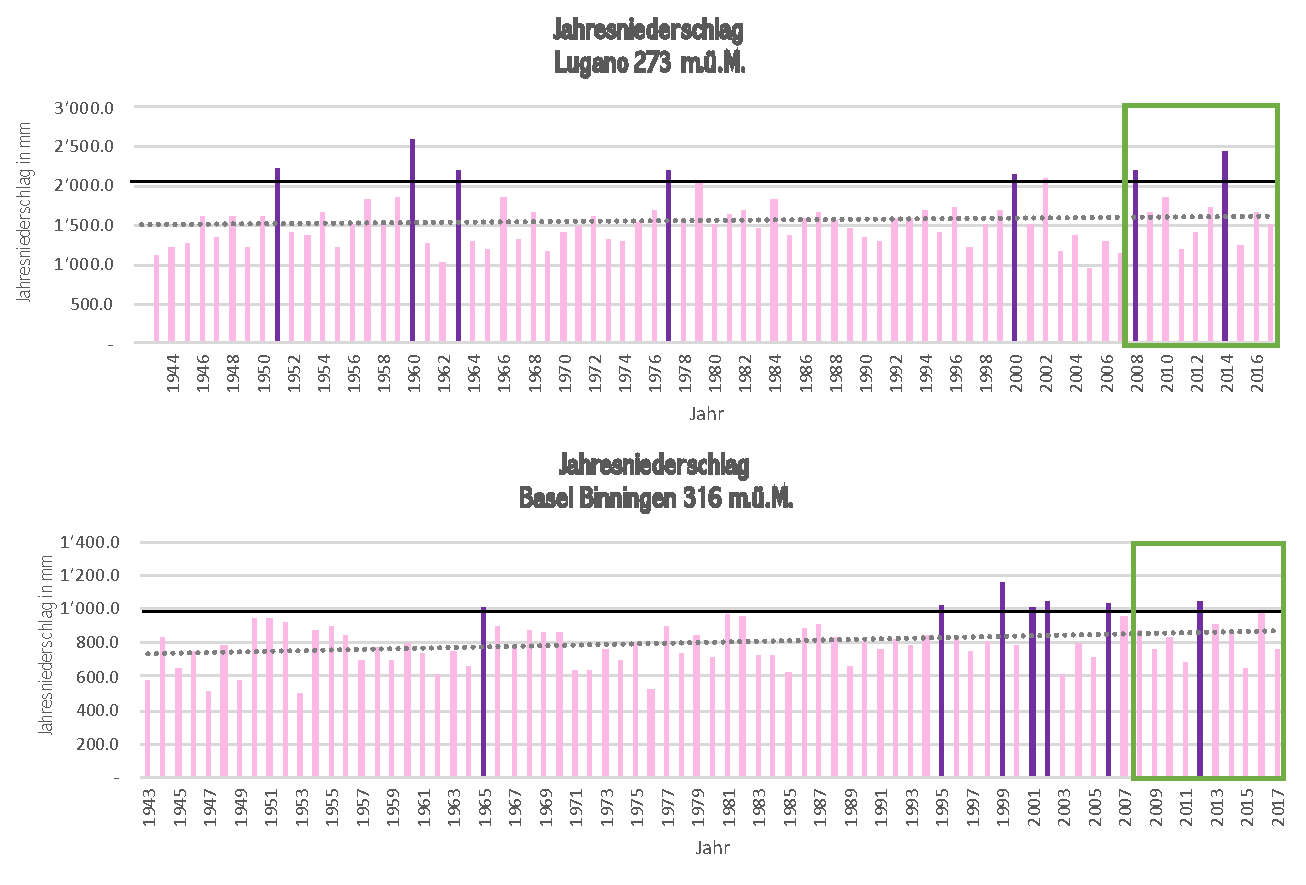
\includegraphics[width=0.8\textwidth]{extrem/Jahresniederschlag.pdf}
\caption{Der Jahresniederschlag gemessen in Millimeter pro Jahr. In den letzten 10 Jahren ist es nicht zu einer Häufung von extremen Ereignissen gekommen. Der Klimawandel wird nicht nachgewiesen.}
\label{Jahresniederschlag}
\end{figure}


\begin{figure}
\centering
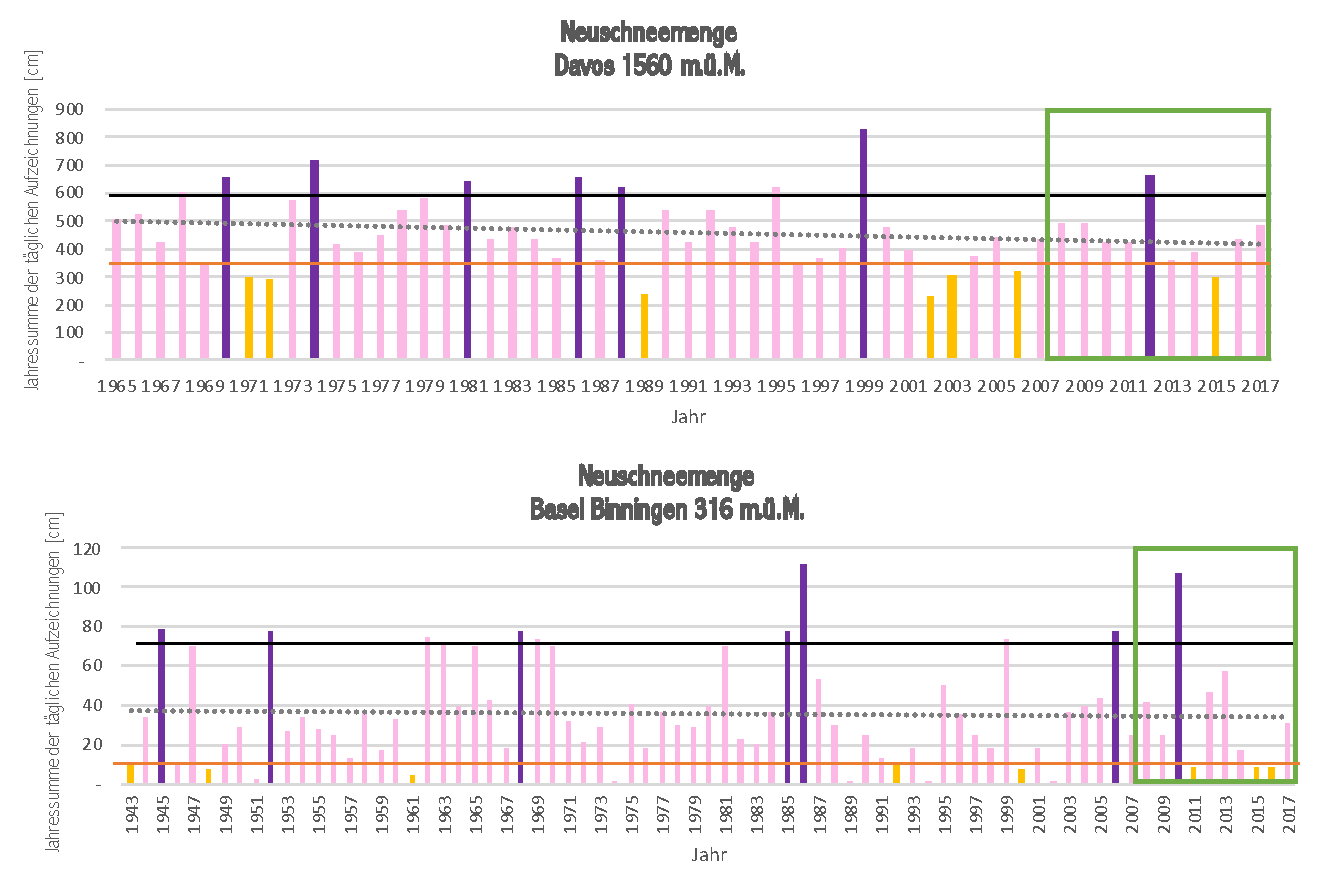
\includegraphics[width=0.8\textwidth]{extrem/Neuschnee.pdf}
\caption{Der Neuschnee gemessen in der Jahressumme an gefallenem Schnee, weisst wie der Jahresniederschlag keine Extremen in den letzten 10 Jahren auf, welche dem Klimawandel zugesprochen werden könnten.}
\label{Neuschnee}
\end{figure}


\begin{figure}
\centering
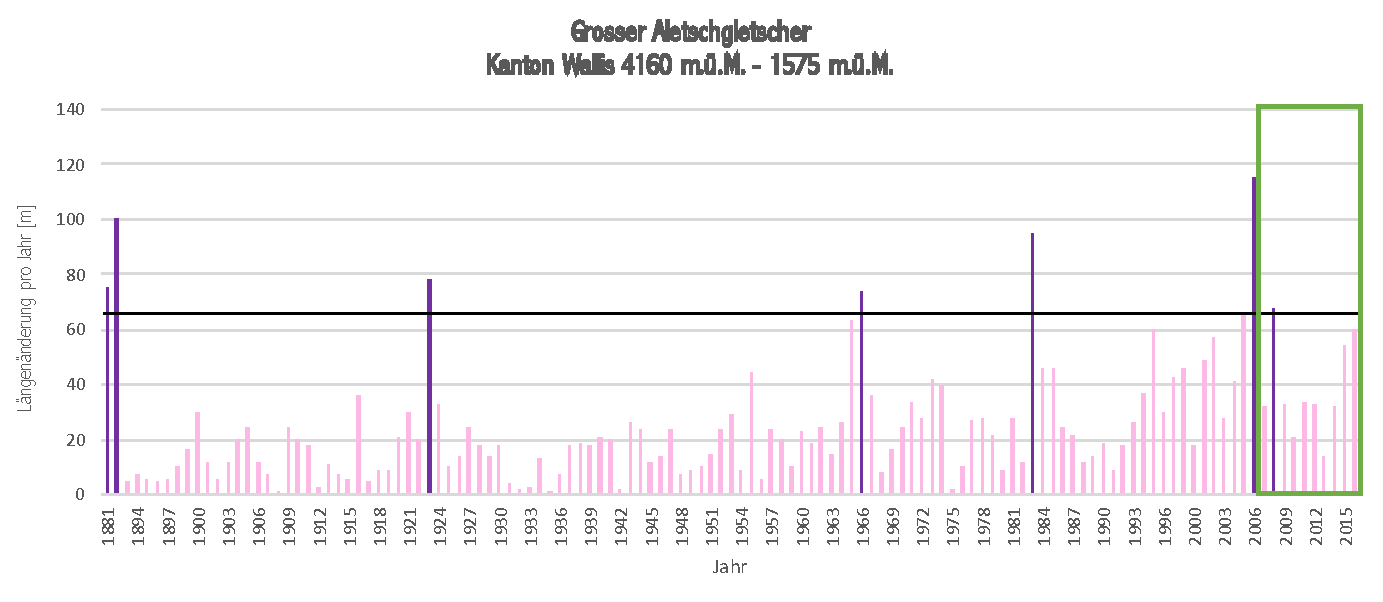
\includegraphics[width=1.0\textwidth]{extrem/Aletsch.pdf}
\caption{Die Längenänderung pro Jahr zeigt beim Aletschgletscher keine auffälligen oder gehäuften extreme Schmelzphasen. Somit kann kein Klimawandel nachgewiesen werden.}
\label{AletschTab}
\end{figure}


\begin{figure}
\centering
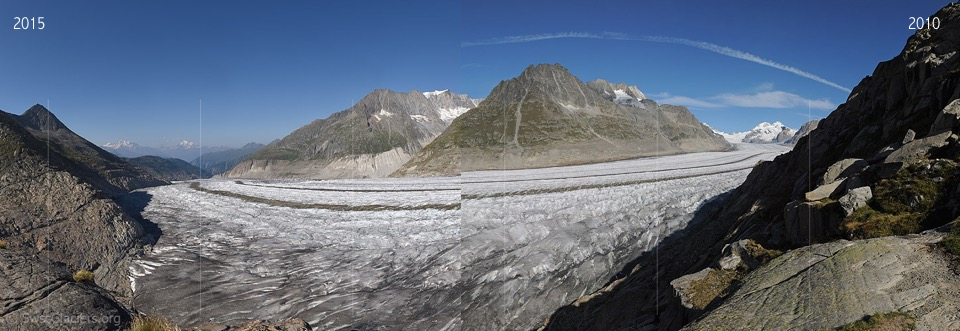
\includegraphics[width=1.0\textwidth]{extrem/Aletsch.jpg}
\caption{Der grosse Aletschgletscher im Wandel der Zeit. Links im Jahr 2015 und rechts im Jahr 2010. Die Volumenänderung ist deutlich ersichtlich.}
\label{Aletsch}
\end{figure}


\begin{figure}
\centering
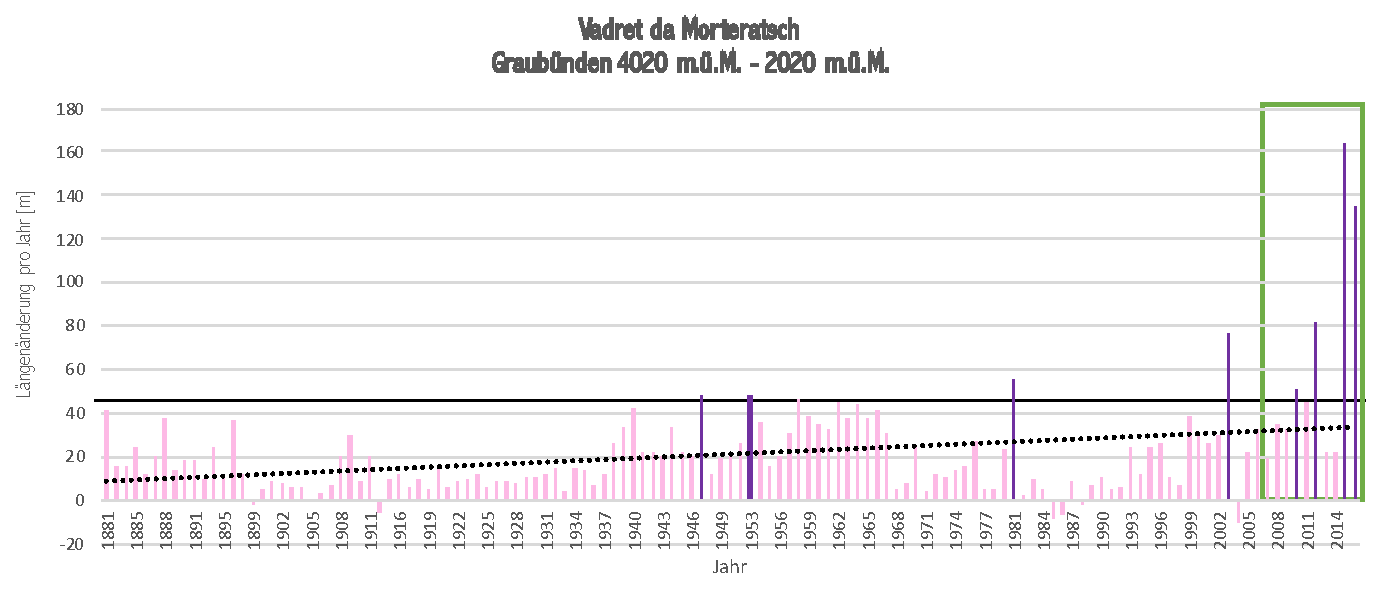
\includegraphics[width=1.0\textwidth]{extrem/Morteratsch.pdf}
\caption{Die Längenänderung pro Jahr zeigt beim Morteratschgletscher deutliche extreme Ereignisse auf. Der Einfluss auf die Längenänderung ist ganz deutlich dem Klimawandel zuzuschreiben. Bemerkenswert ist das Jahr 2004, denn der Morteratschgletscher ist in diesem Jahr um 10 Meter gewachsen.}
\label{Morteratschtab}
\end{figure}


\begin{figure}
\centering
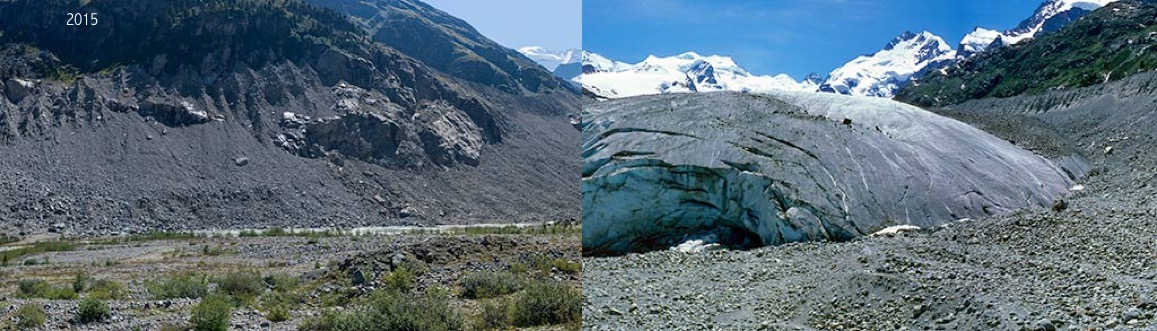
\includegraphics[width=1.0\textwidth]{extrem/Morteratsch.jpg}
\caption{Der Morteratschgletscher im Wandel der Zeit. Links im Jahr 2015 und rechts im Jahr 1985. Die starke Abnahme des Volumens und vor allem die Längenänderung ist unverkennbar.}
\label{Morteratsch}
\end{figure}






\printbibliography[heading=subbibliography]
\end{refsection}
